\section{Method}
\subsection{Oscillator - 555 Timer IC}
\label{sec:555}
The first attempt made for the oscillators is to use a 555 timer chip to directly create an audible frequency square wave signal. The frequency of the 555 IC is determined by the size of the resistances, $R_1$ and $R_2$, and the capacitor, $C$, as located in figure~\ref{fig:555}.

\begin{figure}[htbp]
	\begin{center}
		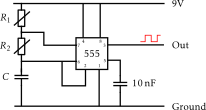
\includegraphics[scale=1.2]{report_img/555}
		\caption{Circuit diagram of the 555 timer IC with the immediate components used to make a VCO.}
		\label{fig:555}
	\end{center}
\end{figure}

The signal is generated by the chip using a series of capacitors and components contained within, a circuit diagram for the 555 can be seen in appendix~\ref{app:555}. The chip is connected in the astable mode so that the output signal is a continuous stream of rectangular pulses with a given frequency that obey equations (\ref{eqn:555freq}), (\ref{eqn:555high}) and (\ref{eqn:555low}), where $\tau_{\text{high}}$ is the time spent in the high voltage position and $\tau_{\text{low}}$ is the low time.\cite{NE555}
\begin{align}
	\label{eqn:555freq}
	f &= \frac{1}{\ln{2}C(R_1+R_2)}, \\
	\label{eqn:555high}
	\tau_{\text{high}} &= \ln{2}C(R_1+R_2), \\
	\label{eqn:555low}
	\tau_{\text{low}} &= \ln{2}CR_2. 
\end{align}
With two chips combined, a high degree of control over the output can be achieved by varying the value of the resistors. As a proof of concept, the circuit in figure \ref{fig:2x555} was built and a variable resistor in the form of an LDR was added. This allowed the pitch and volume to be controlled remotely using the fingers.

\begin{figure}[htbp]
	\begin{center}
		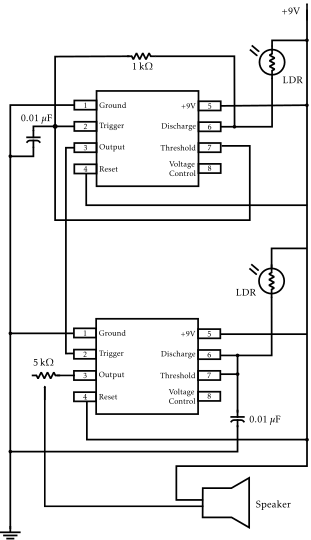
\includegraphics[scale=0.8,angle=90]{report_img/2x555}
		\caption{Circuit diagram of the two 555 timer ICs used to make a rudimentary resistance controlled theremin.}
		\label{fig:2x555}
	\end{center}
\end{figure}

\subsection{Oscillator - HEF4046 IC}
\label{sec:4046}
Though a controllable waveform in the audible frequency range was produced using the previously described 555 timer method, the sound was not pleasant as the wave was square shape and so does not resemble the ideal sinusoidal sound wave. In an attempt to improve the quality of this sound, an alternative VCO chip is tried. The first choice is the 8068 chip but this is no longer in commercial production, so a close relative, the 4046 chip, is used.

This chip contains several components that shall not be used, but importantly has a voltage controlled oscillator that can be used independently. The circuit diagram is shown in appendix~\ref{app:4046}. Pins 4, 6, 7, 10, 13, 15 and 16 are used with others left open.

Under these conditions, with a capacitance of 10\,nF and resistance of 10\,k$\Omega$, an audible sound was produced, shown, as measured on an oscilloscope, in figure~\ref{fig:4046square}.

\begin{figure}[htbp]
	\centering
		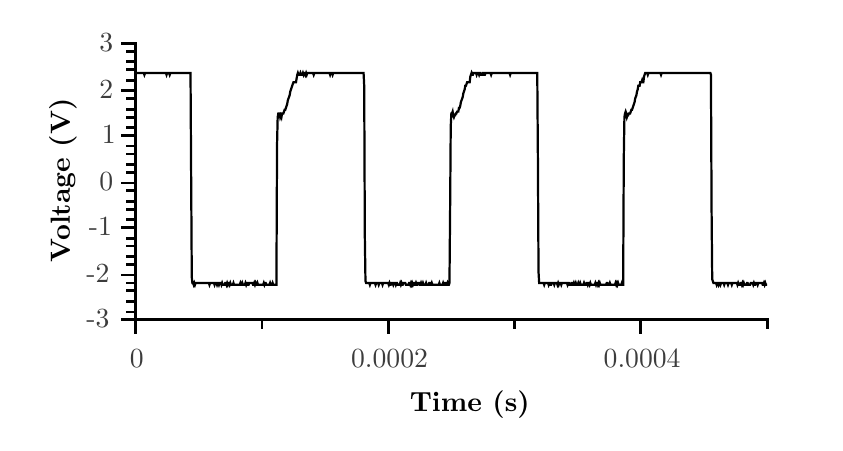
\begin{tikzpicture}{0pt}{0pt}{299pt}{150pt}
	\clip(0pt,150pt) -- (284.325pt,150pt) -- (284.325pt,7.36184pt) -- (0pt,7.36184pt) -- (0pt,150pt);
\begin{scope}
	\clip(38.9878pt,144.294pt) -- (267.209pt,144.294pt) -- (267.209pt,44.4478pt) -- (38.9878pt,44.4478pt) -- (38.9878pt,144.294pt);
	\color[gray]{0}
	\draw[line width=0.8pt, line join=miter, line cap=rect](39.216pt,133.644pt) -- (39.4442pt,133.644pt) -- (39.6724pt,133.644pt) -- (39.9006pt,133.644pt) -- (40.1289pt,133.644pt) -- (40.3571pt,133.644pt) -- (40.5853pt,133.644pt) -- (40.8135pt,133.644pt) -- (41.0418pt,133.644pt) -- (41.27pt,133.644pt) -- (41.4982pt,133.644pt) -- (41.7264pt,133.644pt) -- (41.9546pt,133.644pt) -- (42.1829pt,132.979pt) -- (42.4111pt,133.644pt) -- (42.6393pt,133.644pt) -- (42.8675pt,133.644pt) -- (43.0957pt,133.644pt) -- (43.324pt,133.644pt) -- (43.5522pt,133.644pt) -- (43.7804pt,133.644pt) -- (44.0086pt,133.644pt) -- (44.2368pt,133.644pt) -- (44.4651pt,133.644pt) -- (44.6933pt,133.644pt) -- (44.9215pt,133.644pt) -- (45.1497pt,133.644pt) -- (45.378pt,133.644pt) -- (45.6062pt,133.644pt) -- (45.8344pt,133.644pt) -- (46.0626pt,133.644pt) -- (46.2908pt,133.644pt) -- (46.5191pt,133.644pt) -- (46.7473pt,133.644pt) -- (46.9755pt,133.644pt) -- (47.2037pt,133.644pt) -- (47.4319pt,133.644pt) -- (47.6602pt,133.644pt) -- (47.8884pt,133.644pt) -- (48.1166pt,133.644pt) -- (48.3448pt,133.644pt) -- (48.573pt,133.644pt) -- (48.8013pt,133.644pt) -- (49.0295pt,133.644pt) -- (49.2577pt,133.644pt) -- (49.4859pt,133.644pt) -- (49.7142pt,133.644pt) -- (49.9424pt,133.644pt) -- (50.1706pt,132.979pt) -- (50.3988pt,133.644pt) -- (50.627pt,133.644pt) -- (50.8553pt,133.644pt) -- (51.0835pt,133.644pt) -- (51.3117pt,132.979pt) -- (51.5399pt,133.644pt) -- (51.7681pt,133.644pt) -- (51.9964pt,133.644pt) -- (52.2246pt,133.644pt) -- (52.4528pt,133.644pt) -- (52.681pt,133.644pt) -- (52.9092pt,133.644pt) -- (53.1375pt,133.644pt) -- (53.3657pt,133.644pt) -- (53.5939pt,133.644pt) -- (53.8221pt,133.644pt) -- (54.0504pt,133.644pt) -- (54.2786pt,133.644pt) -- (54.5068pt,133.644pt) -- (54.735pt,133.644pt) -- (54.9632pt,133.644pt) -- (55.1915pt,133.644pt) -- (55.4197pt,133.644pt) -- (55.6479pt,133.644pt) -- (55.8761pt,133.644pt) -- (56.1043pt,133.644pt) -- (56.3326pt,133.644pt) -- (56.5608pt,133.644pt) -- (56.789pt,133.644pt) -- (57.0172pt,133.644pt) -- (57.2454pt,133.644pt) -- (57.4737pt,133.644pt) -- (57.7019pt,133.644pt) -- (57.9301pt,133.644pt) -- (58.1583pt,133.644pt) -- (58.3866pt,133.644pt) -- (58.6148pt,133.644pt) -- (58.843pt,133.644pt) -- (59.0712pt,95.7024pt) -- (59.2994pt,59.7576pt) -- (59.5277pt,57.7607pt) -- (59.7559pt,57.7607pt) -- (59.9841pt,57.095pt) -- (60.2123pt,57.7607pt) -- (60.4405pt,57.095pt) -- (60.6688pt,57.7607pt) -- (60.897pt,57.7607pt) -- (61.1252pt,57.7607pt) -- (61.3534pt,57.7607pt) -- (61.5816pt,57.7607pt) -- (61.8099pt,57.7607pt) -- (62.0381pt,57.7607pt) -- (62.2663pt,57.7607pt) -- (62.4945pt,57.7607pt) -- (62.7228pt,57.7607pt) -- (62.951pt,57.7607pt) -- (63.1792pt,57.7607pt) -- (63.4074pt,57.7607pt) -- (63.6356pt,57.7607pt) -- (63.8639pt,57.7607pt) -- (64.0921pt,57.7607pt) -- (64.3203pt,57.7607pt) -- (64.5485pt,57.7607pt) -- (64.7767pt,57.7607pt) -- (65.005pt,57.7607pt) -- (65.2332pt,57.7607pt) -- (65.4614pt,57.7607pt) -- (65.6896pt,57.095pt) -- (65.9178pt,57.7607pt) -- (66.1461pt,57.7607pt) -- (66.3743pt,57.7607pt) -- (66.6025pt,57.7607pt) -- (66.8307pt,57.7607pt) -- (67.059pt,57.7607pt) -- (67.2872pt,57.7607pt) -- (67.5154pt,57.095pt) -- (67.7436pt,57.7607pt) -- (67.9718pt,57.7607pt) -- (68.2001pt,57.7607pt) -- (68.4283pt,57.095pt) -- (68.6565pt,57.7607pt) -- (68.8847pt,57.7607pt) -- (69.1129pt,57.095pt) -- (69.3412pt,57.7607pt) -- (69.5694pt,57.7607pt) -- (69.7976pt,57.7607pt) -- (70.0258pt,57.095pt) -- (70.254pt,57.7607pt) -- (70.4823pt,57.095pt) -- (70.7105pt,57.095pt) -- (70.9387pt,57.095pt) -- (71.1669pt,57.095pt) -- (71.3952pt,57.7607pt) -- (71.6234pt,57.7607pt) -- (71.8516pt,57.095pt) -- (72.0798pt,57.7607pt) -- (72.308pt,57.095pt) -- (72.5363pt,57.7607pt) -- (72.7645pt,57.7607pt) -- (72.9927pt,57.095pt) -- (73.2209pt,57.7607pt) -- (73.4491pt,57.095pt) -- (73.6774pt,57.095pt) -- (73.9056pt,57.095pt) -- (74.1338pt,57.095pt) -- (74.362pt,57.7607pt) -- (74.5902pt,57.095pt) -- (74.8185pt,57.095pt) -- (75.0467pt,57.095pt) -- (75.2749pt,57.095pt) -- (75.5031pt,57.095pt) -- (75.7314pt,57.095pt) -- (75.9596pt,57.095pt) -- (76.1878pt,57.095pt) -- (76.416pt,57.095pt) -- (76.6442pt,57.095pt) -- (76.8725pt,57.7607pt) -- (77.1007pt,57.095pt) -- (77.3289pt,57.095pt) -- (77.5571pt,57.7607pt) -- (77.7853pt,57.095pt) -- (78.0136pt,57.095pt) -- (78.2418pt,57.095pt) -- (78.47pt,57.095pt) -- (78.6982pt,57.7607pt) -- (78.9264pt,57.095pt) -- (79.1547pt,57.7607pt) -- (79.3829pt,57.7607pt) -- (79.6111pt,57.095pt) -- (79.8393pt,57.095pt) -- (80.0676pt,57.7607pt) -- (80.2958pt,57.7607pt) -- (80.524pt,57.7607pt) -- (80.7522pt,57.7607pt) -- (80.9804pt,57.7607pt) -- (81.2087pt,57.7607pt) -- (81.4369pt,57.095pt) -- (81.6651pt,57.095pt) -- (81.8933pt,57.7607pt) -- (82.1215pt,57.095pt) -- (82.3498pt,57.7607pt) -- (82.578pt,57.095pt) -- (82.8062pt,57.095pt) -- (83.0344pt,57.7607pt) -- (83.2626pt,57.095pt) -- (83.4909pt,57.095pt) -- (83.7191pt,57.095pt) -- (83.9473pt,57.095pt) -- (84.1755pt,57.095pt) -- (84.4038pt,57.095pt) -- (84.632pt,57.095pt) -- (84.8602pt,57.095pt) -- (85.0884pt,57.095pt) -- (85.3166pt,57.7607pt) -- (85.5449pt,57.095pt) -- (85.7731pt,57.7607pt) -- (86.0013pt,57.7607pt) -- (86.2295pt,57.095pt) -- (86.4577pt,57.095pt) -- (86.686pt,57.095pt) -- (86.9142pt,57.095pt) -- (87.1424pt,57.095pt) -- (87.3706pt,57.095pt) -- (87.5988pt,57.7607pt) -- (87.8271pt,57.095pt) -- (88.0553pt,57.095pt) -- (88.2835pt,57.095pt) -- (88.5117pt,57.7607pt) -- (88.74pt,57.095pt) -- (88.9682pt,57.095pt) -- (89.1964pt,57.095pt) -- (89.4246pt,57.095pt) -- (89.6528pt,57.095pt) -- (89.8811pt,57.095pt) -- (90.1093pt,107.684pt) -- (90.3375pt,117.669pt) -- (90.5657pt,119pt) -- (90.7939pt,119pt) -- (91.0222pt,119pt) -- (91.2504pt,117.669pt) -- (91.4786pt,118.334pt) -- (91.7068pt,117.669pt) -- (91.935pt,119pt) -- (92.1633pt,119pt) -- (92.3915pt,119pt) -- (92.6197pt,119.666pt) -- (92.8479pt,120.331pt) -- (93.0762pt,120.331pt) -- (93.3044pt,120.997pt) -- (93.5326pt,121.663pt) -- (93.7608pt,122.328pt) -- (93.989pt,123.659pt) -- (94.2173pt,124.325pt) -- (94.4455pt,124.991pt) -- (94.6737pt,125.656pt) -- (94.9019pt,126.988pt) -- (95.1301pt,127.653pt) -- (95.3584pt,128.319pt) -- (95.5866pt,128.985pt) -- (95.8148pt,129.65pt) -- (96.043pt,130.316pt) -- (96.2712pt,130.316pt) -- (96.4995pt,130.316pt) -- (96.7277pt,130.316pt) -- (96.9559pt,130.316pt) -- (97.1841pt,131.647pt) -- (97.4124pt,132.979pt) -- (97.6406pt,133.644pt) -- (97.8688pt,132.979pt) -- (98.097pt,132.979pt) -- (98.3252pt,132.979pt) -- (98.5535pt,133.644pt) -- (98.7817pt,132.979pt) -- (99.0099pt,132.979pt) -- (99.2381pt,132.979pt) -- (99.4663pt,133.644pt) -- (99.6946pt,132.979pt) -- (99.9228pt,133.644pt) -- (100.151pt,133.644pt) -- (100.379pt,132.979pt) -- (100.607pt,133.644pt) -- (100.836pt,132.979pt) -- (101.064pt,133.644pt) -- (101.292pt,133.644pt) -- (101.52pt,133.644pt) -- (101.749pt,133.644pt) -- (101.977pt,133.644pt) -- (102.205pt,133.644pt) -- (102.433pt,133.644pt) -- (102.661pt,133.644pt) -- (102.89pt,133.644pt) -- (103.118pt,133.644pt) -- (103.346pt,132.979pt) -- (103.574pt,133.644pt) -- (103.803pt,133.644pt) -- (104.031pt,133.644pt) -- (104.259pt,133.644pt) -- (104.487pt,133.644pt) -- (104.715pt,133.644pt) -- (104.944pt,133.644pt) -- (105.172pt,133.644pt) -- (105.4pt,133.644pt) -- (105.628pt,133.644pt) -- (105.857pt,133.644pt) -- (106.085pt,133.644pt) -- (106.313pt,133.644pt) -- (106.541pt,133.644pt) -- (106.769pt,133.644pt) -- (106.998pt,133.644pt) -- (107.226pt,133.644pt) -- (107.454pt,133.644pt) -- (107.682pt,133.644pt) -- (107.911pt,133.644pt) -- (108.139pt,133.644pt) -- (108.367pt,133.644pt) -- (108.595pt,133.644pt) -- (108.823pt,133.644pt) -- (109.052pt,133.644pt) -- (109.28pt,132.979pt) -- (109.508pt,133.644pt) -- (109.736pt,133.644pt) -- (109.965pt,133.644pt) -- (110.193pt,132.979pt) -- (110.421pt,133.644pt) -- (110.649pt,133.644pt) -- (110.877pt,133.644pt) -- (111.106pt,133.644pt) -- (111.334pt,133.644pt) -- (111.562pt,133.644pt) -- (111.79pt,133.644pt) -- (112.019pt,133.644pt) -- (112.247pt,133.644pt) -- (112.475pt,133.644pt) -- (112.703pt,133.644pt) -- (112.931pt,133.644pt) -- (113.16pt,133.644pt) -- (113.388pt,133.644pt) -- (113.616pt,133.644pt) -- (113.844pt,133.644pt) -- (114.072pt,133.644pt) -- (114.301pt,133.644pt) -- (114.529pt,133.644pt) -- (114.757pt,133.644pt) -- (114.985pt,133.644pt) -- (115.214pt,133.644pt) -- (115.442pt,133.644pt) -- (115.67pt,133.644pt) -- (115.898pt,133.644pt) -- (116.126pt,133.644pt) -- (116.355pt,133.644pt) -- (116.583pt,133.644pt) -- (116.811pt,133.644pt) -- (117.039pt,133.644pt) -- (117.268pt,133.644pt) -- (117.496pt,133.644pt) -- (117.724pt,133.644pt) -- (117.952pt,133.644pt) -- (118.18pt,133.644pt) -- (118.409pt,133.644pt) -- (118.637pt,133.644pt) -- (118.865pt,133.644pt) -- (119.093pt,133.644pt) -- (119.322pt,133.644pt) -- (119.55pt,133.644pt) -- (119.778pt,133.644pt) -- (120.006pt,133.644pt) -- (120.234pt,133.644pt) -- (120.463pt,133.644pt) -- (120.691pt,133.644pt) -- (120.919pt,133.644pt) -- (121.147pt,133.644pt) -- (121.376pt,133.644pt) -- (121.604pt,128.985pt) -- (121.832pt,74.4018pt) -- (122.06pt,58.4263pt) -- (122.288pt,57.7607pt) -- (122.517pt,57.7607pt) -- (122.745pt,57.7607pt) -- (122.973pt,57.7607pt) -- (123.201pt,57.7607pt) -- (123.43pt,57.7607pt) -- (123.658pt,57.095pt) -- (123.886pt,57.7607pt) -- (124.114pt,57.7607pt) -- (124.342pt,57.7607pt) -- (124.571pt,57.7607pt) -- (124.799pt,57.7607pt) -- (125.027pt,57.7607pt) -- (125.255pt,57.7607pt) -- (125.484pt,57.7607pt) -- (125.712pt,57.095pt) -- (125.94pt,57.7607pt) -- (126.168pt,57.7607pt) -- (126.396pt,57.7607pt) -- (126.625pt,57.7607pt) -- (126.853pt,57.095pt) -- (127.081pt,57.7607pt) -- (127.309pt,57.7607pt) -- (127.538pt,57.7607pt) -- (127.766pt,57.7607pt) -- (127.994pt,57.7607pt) -- (128.222pt,57.095pt) -- (128.45pt,57.7607pt) -- (128.679pt,57.7607pt) -- (128.907pt,57.7607pt) -- (129.135pt,57.7607pt) -- (129.363pt,57.7607pt) -- (129.592pt,57.7607pt) -- (129.82pt,57.7607pt) -- (130.048pt,57.7607pt) -- (130.276pt,57.7607pt) -- (130.504pt,57.095pt) -- (130.733pt,57.7607pt) -- (130.961pt,57.095pt) -- (131.189pt,57.095pt) -- (131.417pt,57.7607pt) -- (131.646pt,57.7607pt) -- (131.874pt,57.7607pt) -- (132.102pt,57.095pt) -- (132.33pt,57.7607pt) -- (132.558pt,57.7607pt) -- (132.787pt,57.7607pt) -- (133.015pt,57.095pt) -- (133.243pt,57.7607pt) -- (133.471pt,57.7607pt) -- (133.7pt,57.095pt) -- (133.928pt,57.095pt) -- (134.156pt,57.095pt) -- (134.384pt,57.095pt) -- (134.612pt,57.7607pt) -- (134.841pt,57.095pt) -- (135.069pt,57.7607pt) -- (135.297pt,57.095pt) -- (135.525pt,57.095pt) -- (135.753pt,57.7607pt) -- (135.982pt,57.7607pt) -- (136.21pt,57.7607pt) -- (136.438pt,57.7607pt) -- (136.666pt,57.095pt) -- (136.895pt,57.095pt) -- (137.123pt,57.095pt) -- (137.351pt,57.095pt) -- (137.579pt,57.095pt) -- (137.807pt,57.7607pt) -- (138.036pt,57.7607pt) -- (138.264pt,57.095pt) -- (138.492pt,57.7607pt) -- (138.72pt,57.095pt) -- (138.949pt,57.7607pt) -- (139.177pt,57.095pt) -- (139.405pt,57.7607pt) -- (139.633pt,57.7607pt) -- (139.861pt,57.095pt) -- (140.09pt,57.095pt) -- (140.318pt,57.7607pt) -- (140.546pt,57.095pt) -- (140.774pt,57.095pt) -- (141.003pt,57.7607pt) -- (141.231pt,57.7607pt) -- (141.459pt,57.7607pt) -- (141.687pt,57.095pt) -- (141.915pt,57.095pt) -- (142.144pt,57.7607pt) -- (142.372pt,57.095pt) -- (142.6pt,57.095pt) -- (142.828pt,57.7607pt) -- (143.057pt,57.095pt) -- (143.285pt,57.095pt) -- (143.513pt,57.095pt) -- (143.741pt,57.095pt) -- (143.969pt,57.7607pt) -- (144.198pt,57.095pt) -- (144.426pt,57.095pt) -- (144.654pt,57.095pt) -- (144.882pt,57.095pt) -- (145.111pt,57.7607pt) -- (145.339pt,57.7607pt) -- (145.567pt,57.095pt) -- (145.795pt,57.095pt) -- (146.023pt,57.7607pt) -- (146.252pt,57.095pt) -- (146.48pt,57.095pt) -- (146.708pt,57.095pt) -- (146.936pt,57.095pt) -- (147.165pt,57.095pt) -- (147.393pt,57.095pt) -- (147.621pt,57.095pt) -- (147.849pt,57.095pt) -- (148.077pt,57.095pt) -- (148.306pt,57.095pt) -- (148.534pt,57.095pt) -- (148.762pt,57.7607pt) -- (148.99pt,57.095pt) -- (149.219pt,57.095pt) -- (149.447pt,57.095pt) -- (149.675pt,57.095pt) -- (149.903pt,57.095pt) -- (150.131pt,57.7607pt) -- (150.36pt,57.095pt) -- (150.588pt,57.095pt) -- (150.816pt,57.7607pt) -- (151.044pt,57.7607pt) -- (151.273pt,57.095pt) -- (151.501pt,57.095pt) -- (151.729pt,57.7607pt) -- (151.957pt,57.095pt) -- (152.185pt,57.095pt) -- (152.414pt,57.7607pt) -- (152.642pt,83.7208pt) -- (152.87pt,114.34pt) -- (153.098pt,119pt) -- (153.327pt,119pt) -- (153.555pt,119.666pt) -- (153.783pt,118.334pt) -- (154.011pt,117.669pt) -- (154.239pt,118.334pt) -- (154.468pt,118.334pt) -- (154.696pt,119pt) -- (154.924pt,119pt) -- (155.152pt,119.666pt) -- (155.38pt,119.666pt) -- (155.609pt,119.666pt) -- (155.837pt,120.997pt) -- (156.065pt,120.997pt) -- (156.293pt,121.663pt) -- (156.522pt,122.994pt) -- (156.75pt,123.659pt) -- (156.978pt,124.325pt) -- (157.206pt,124.991pt) -- (157.434pt,126.322pt) -- (157.663pt,126.988pt) -- (157.891pt,127.653pt) -- (158.119pt,128.985pt) -- (158.347pt,128.985pt) -- (158.576pt,129.65pt) -- (158.804pt,130.316pt) -- (159.032pt,130.316pt) -- (159.26pt,130.316pt) -- (159.488pt,130.316pt) -- (159.717pt,130.316pt) -- (159.945pt,132.313pt) -- (160.173pt,132.979pt) -- (160.401pt,133.644pt) -- (160.63pt,132.979pt) -- (160.858pt,132.979pt) -- (161.086pt,133.644pt) -- (161.314pt,133.644pt) -- (161.542pt,133.644pt) -- (161.771pt,133.644pt) -- (161.999pt,133.644pt) -- (162.227pt,132.979pt) -- (162.455pt,133.644pt) -- (162.684pt,133.644pt) -- (162.912pt,133.644pt) -- (163.14pt,132.979pt) -- (163.368pt,133.644pt) -- (163.596pt,133.644pt) -- (163.825pt,132.979pt) -- (164.053pt,132.979pt) -- (164.281pt,132.979pt) -- (164.509pt,133.644pt) -- (164.738pt,133.644pt) -- (164.966pt,132.979pt) -- (165.194pt,132.979pt) -- (165.422pt,133.644pt) -- (165.65pt,133.644pt) -- (165.879pt,133.644pt) -- (166.107pt,133.644pt) -- (166.335pt,133.644pt) -- (166.563pt,133.644pt) -- (166.792pt,133.644pt) -- (167.02pt,133.644pt) -- (167.248pt,133.644pt) -- (167.476pt,132.979pt) -- (167.704pt,133.644pt) -- (167.933pt,133.644pt) -- (168.161pt,133.644pt) -- (168.389pt,133.644pt) -- (168.617pt,133.644pt) -- (168.846pt,133.644pt) -- (169.074pt,133.644pt) -- (169.302pt,133.644pt) -- (169.53pt,133.644pt) -- (169.758pt,133.644pt) -- (169.987pt,133.644pt) -- (170.215pt,133.644pt) -- (170.443pt,133.644pt) -- (170.671pt,133.644pt) -- (170.9pt,133.644pt) -- (171.128pt,133.644pt) -- (171.356pt,133.644pt) -- (171.584pt,133.644pt) -- (171.812pt,133.644pt) -- (172.041pt,133.644pt) -- (172.269pt,133.644pt) -- (172.497pt,133.644pt) -- (172.725pt,133.644pt) -- (172.954pt,133.644pt) -- (173.182pt,133.644pt) -- (173.41pt,133.644pt) -- (173.638pt,133.644pt) -- (173.866pt,133.644pt) -- (174.095pt,133.644pt) -- (174.323pt,132.979pt) -- (174.551pt,133.644pt) -- (174.779pt,133.644pt) -- (175.008pt,133.644pt) -- (175.236pt,133.644pt) -- (175.464pt,133.644pt) -- (175.692pt,133.644pt) -- (175.92pt,133.644pt) -- (176.149pt,133.644pt) -- (176.377pt,133.644pt) -- (176.605pt,133.644pt) -- (176.833pt,133.644pt) -- (177.061pt,133.644pt) -- (177.29pt,133.644pt) -- (177.518pt,133.644pt) -- (177.746pt,133.644pt) -- (177.974pt,133.644pt) -- (178.203pt,133.644pt) -- (178.431pt,133.644pt) -- (178.659pt,133.644pt) -- (178.887pt,133.644pt) -- (179.115pt,133.644pt) -- (179.344pt,133.644pt) -- (179.572pt,133.644pt) -- (179.8pt,133.644pt) -- (180.028pt,133.644pt) -- (180.257pt,133.644pt) -- (180.485pt,133.644pt) -- (180.713pt,133.644pt) -- (180.941pt,133.644pt) -- (181.169pt,133.644pt) -- (181.398pt,133.644pt) -- (181.626pt,133.644pt) -- (181.854pt,133.644pt) -- (182.082pt,133.644pt) -- (182.311pt,133.644pt) -- (182.539pt,133.644pt) -- (182.767pt,133.644pt) -- (182.995pt,133.644pt) -- (183.223pt,133.644pt) -- (183.452pt,133.644pt) -- (183.68pt,133.644pt) -- (183.908pt,133.644pt) -- (184.136pt,133.644pt) -- (184.365pt,103.025pt) -- (184.593pt,61.7545pt) -- (184.821pt,57.7607pt) -- (185.049pt,57.7607pt) -- (185.277pt,57.7607pt) -- (185.506pt,57.7607pt) -- (185.734pt,57.7607pt) -- (185.962pt,57.7607pt) -- (186.19pt,57.7607pt) -- (186.419pt,57.7607pt) -- (186.647pt,57.095pt) -- (186.875pt,57.7607pt) -- (187.103pt,57.7607pt) -- (187.331pt,57.7607pt) -- (187.56pt,57.7607pt) -- (187.788pt,57.7607pt) -- (188.016pt,57.7607pt) -- (188.244pt,57.095pt) -- (188.473pt,57.7607pt) -- (188.701pt,57.7607pt) -- (188.929pt,57.095pt) -- (189.157pt,57.095pt) -- (189.385pt,57.7607pt) -- (189.614pt,57.7607pt) -- (189.842pt,57.7607pt) -- (190.07pt,57.7607pt) -- (190.298pt,57.095pt) -- (190.527pt,57.7607pt) -- (190.755pt,57.7607pt) -- (190.983pt,57.7607pt) -- (191.211pt,57.7607pt) -- (191.439pt,57.095pt) -- (191.668pt,57.7607pt) -- (191.896pt,57.095pt) -- (192.124pt,57.7607pt) -- (192.352pt,57.7607pt) -- (192.581pt,57.7607pt) -- (192.809pt,57.095pt) -- (193.037pt,57.7607pt) -- (193.265pt,57.7607pt) -- (193.493pt,57.7607pt) -- (193.722pt,57.7607pt) -- (193.95pt,57.7607pt) -- (194.178pt,57.7607pt) -- (194.406pt,57.7607pt) -- (194.635pt,57.7607pt) -- (194.863pt,57.7607pt) -- (195.091pt,57.095pt) -- (195.319pt,57.7607pt) -- (195.547pt,57.7607pt) -- (195.776pt,57.095pt) -- (196.004pt,57.095pt) -- (196.232pt,57.095pt) -- (196.46pt,57.7607pt) -- (196.689pt,57.7607pt) -- (196.917pt,57.095pt) -- (197.145pt,57.095pt) -- (197.373pt,57.7607pt) -- (197.601pt,57.095pt) -- (197.83pt,57.095pt) -- (198.058pt,57.7607pt) -- (198.286pt,57.095pt) -- (198.514pt,57.095pt) -- (198.742pt,57.095pt) -- (198.971pt,57.7607pt) -- (199.199pt,57.095pt) -- (199.427pt,57.095pt) -- (199.655pt,57.7607pt) -- (199.884pt,57.095pt) -- (200.112pt,57.095pt) -- (200.34pt,57.095pt) -- (200.568pt,57.095pt) -- (200.796pt,57.095pt) -- (201.025pt,57.7607pt) -- (201.253pt,57.095pt) -- (201.481pt,57.095pt) -- (201.709pt,57.095pt) -- (201.938pt,57.7607pt) -- (202.166pt,57.7607pt) -- (202.394pt,57.095pt) -- (202.622pt,57.7607pt) -- (202.85pt,57.7607pt) -- (203.079pt,57.095pt) -- (203.307pt,57.7607pt) -- (203.535pt,57.095pt) -- (203.763pt,57.095pt) -- (203.992pt,57.095pt) -- (204.22pt,57.095pt) -- (204.448pt,57.095pt) -- (204.676pt,57.095pt) -- (204.904pt,57.095pt) -- (205.133pt,57.7607pt) -- (205.361pt,57.095pt) -- (205.589pt,57.7607pt) -- (205.817pt,57.7607pt) -- (206.046pt,57.095pt) -- (206.274pt,57.7607pt) -- (206.502pt,57.095pt) -- (206.73pt,57.7607pt) -- (206.958pt,57.095pt) -- (207.187pt,57.095pt) -- (207.415pt,57.095pt) -- (207.643pt,57.095pt) -- (207.871pt,57.095pt) -- (208.1pt,57.095pt) -- (208.328pt,57.095pt) -- (208.556pt,57.095pt) -- (208.784pt,57.095pt) -- (209.012pt,57.095pt) -- (209.241pt,57.7607pt) -- (209.469pt,57.7607pt) -- (209.697pt,57.095pt) -- (209.925pt,57.095pt) -- (210.154pt,57.095pt) -- (210.382pt,57.7607pt) -- (210.61pt,57.095pt) -- (210.838pt,57.095pt) -- (211.066pt,57.095pt) -- (211.295pt,57.095pt) -- (211.523pt,57.095pt) -- (211.751pt,57.095pt) -- (211.979pt,57.095pt) -- (212.208pt,57.095pt) -- (212.436pt,57.7607pt) -- (212.664pt,57.095pt) -- (212.892pt,57.7607pt) -- (213.12pt,57.095pt) -- (213.349pt,57.7607pt) -- (213.577pt,57.095pt) -- (213.805pt,57.095pt) -- (214.033pt,57.095pt) -- (214.262pt,57.095pt) -- (214.49pt,57.095pt) -- (214.718pt,57.7607pt) -- (214.946pt,57.095pt) -- (215.174pt,57.095pt) -- (215.403pt,103.025pt) -- (215.631pt,117.669pt) -- (215.859pt,119pt) -- (216.087pt,119.666pt) -- (216.316pt,119pt) -- (216.544pt,117.669pt) -- (216.772pt,118.334pt) -- (217pt,118.334pt) -- (217.228pt,119pt) -- (217.457pt,119pt) -- (217.685pt,119pt) -- (217.913pt,119.666pt) -- (218.141pt,120.331pt) -- (218.37pt,120.331pt) -- (218.598pt,120.997pt) -- (218.826pt,121.663pt) -- (219.054pt,122.328pt) -- (219.282pt,122.994pt) -- (219.511pt,124.325pt) -- (219.739pt,124.991pt) -- (219.967pt,125.656pt) -- (220.195pt,126.988pt) -- (220.423pt,127.653pt) -- (220.652pt,128.985pt) -- (220.88pt,128.985pt) -- (221.108pt,128.985pt) -- (221.336pt,130.316pt) -- (221.565pt,130.316pt) -- (221.793pt,130.316pt) -- (222.021pt,130.982pt) -- (222.249pt,130.316pt) -- (222.477pt,130.316pt) -- (222.706pt,132.313pt) -- (222.934pt,132.979pt) -- (223.162pt,133.644pt) -- (223.39pt,133.644pt) -- (223.619pt,133.644pt) -- (223.847pt,133.644pt) -- (224.075pt,132.979pt) -- (224.303pt,133.644pt) -- (224.531pt,133.644pt) -- (224.76pt,133.644pt) -- (224.988pt,133.644pt) -- (225.216pt,133.644pt) -- (225.444pt,133.644pt) -- (225.673pt,133.644pt) -- (225.901pt,133.644pt) -- (226.129pt,133.644pt) -- (226.357pt,133.644pt) -- (226.585pt,133.644pt) -- (226.814pt,133.644pt) -- (227.042pt,133.644pt) -- (227.27pt,133.644pt) -- (227.498pt,133.644pt) -- (227.727pt,133.644pt) -- (227.955pt,133.644pt) -- (228.183pt,133.644pt) -- (228.411pt,133.644pt) -- (228.639pt,133.644pt) -- (228.868pt,132.979pt) -- (229.096pt,133.644pt) -- (229.324pt,133.644pt) -- (229.552pt,133.644pt) -- (229.781pt,133.644pt) -- (230.009pt,133.644pt) -- (230.237pt,133.644pt) -- (230.465pt,133.644pt) -- (230.693pt,133.644pt) -- (230.922pt,133.644pt) -- (231.15pt,133.644pt) -- (231.378pt,133.644pt) -- (231.606pt,133.644pt) -- (231.835pt,133.644pt) -- (232.063pt,133.644pt) -- (232.291pt,133.644pt) -- (232.519pt,133.644pt) -- (232.747pt,133.644pt) -- (232.976pt,133.644pt) -- (233.204pt,133.644pt) -- (233.432pt,133.644pt) -- (233.66pt,133.644pt) -- (233.889pt,133.644pt) -- (234.117pt,133.644pt) -- (234.345pt,133.644pt) -- (234.573pt,133.644pt) -- (234.801pt,133.644pt) -- (235.03pt,133.644pt) -- (235.258pt,133.644pt) -- (235.486pt,133.644pt) -- (235.714pt,133.644pt) -- (235.943pt,133.644pt) -- (236.171pt,133.644pt) -- (236.399pt,133.644pt) -- (236.627pt,133.644pt) -- (236.855pt,133.644pt) -- (237.084pt,133.644pt) -- (237.312pt,133.644pt) -- (237.54pt,133.644pt) -- (237.768pt,133.644pt) -- (237.997pt,133.644pt) -- (238.225pt,133.644pt) -- (238.453pt,133.644pt) -- (238.681pt,133.644pt) -- (238.909pt,133.644pt) -- (239.138pt,133.644pt) -- (239.366pt,133.644pt) -- (239.594pt,133.644pt) -- (239.822pt,133.644pt) -- (240.051pt,133.644pt) -- (240.279pt,133.644pt) -- (240.507pt,133.644pt) -- (240.735pt,133.644pt) -- (240.963pt,133.644pt) -- (241.192pt,133.644pt) -- (241.42pt,133.644pt) -- (241.648pt,133.644pt) -- (241.876pt,133.644pt) -- (242.104pt,133.644pt) -- (242.333pt,133.644pt) -- (242.561pt,133.644pt) -- (242.789pt,133.644pt) -- (243.017pt,133.644pt) -- (243.246pt,133.644pt) -- (243.474pt,133.644pt) -- (243.702pt,133.644pt) -- (243.93pt,133.644pt) -- (244.158pt,133.644pt) -- (244.387pt,133.644pt) -- (244.615pt,133.644pt) -- (244.843pt,133.644pt) -- (245.071pt,133.644pt) -- (245.3pt,133.644pt) -- (245.528pt,133.644pt) -- (245.756pt,133.644pt) -- (245.984pt,133.644pt) -- (246.212pt,133.644pt) -- (246.441pt,133.644pt) -- (246.669pt,133.644pt) -- (246.897pt,132.979pt) -- (247.125pt,84.3864pt) -- (247.354pt,59.0919pt) -- (247.582pt,58.4263pt) -- (247.81pt,57.7607pt) -- (248.038pt,57.7607pt) -- (248.266pt,57.7607pt) -- (248.495pt,57.7607pt) -- (248.723pt,57.7607pt) -- (248.951pt,57.095pt) -- (249.179pt,57.7607pt) -- (249.408pt,57.7607pt) -- (249.636pt,57.095pt) -- (249.864pt,57.7607pt) -- (250.092pt,57.7607pt) -- (250.32pt,57.095pt) -- (250.549pt,57.7607pt) -- (250.777pt,57.7607pt) -- (251.005pt,57.7607pt) -- (251.233pt,57.7607pt) -- (251.462pt,57.7607pt) -- (251.69pt,57.095pt) -- (251.918pt,57.7607pt) -- (252.146pt,57.7607pt) -- (252.374pt,57.7607pt) -- (252.603pt,57.7607pt) -- (252.831pt,57.7607pt) -- (253.059pt,57.095pt) -- (253.287pt,57.7607pt) -- (253.516pt,57.7607pt) -- (253.744pt,57.7607pt) -- (253.972pt,57.7607pt) -- (254.2pt,57.7607pt) -- (254.428pt,57.095pt) -- (254.657pt,57.7607pt) -- (254.885pt,57.7607pt) -- (255.113pt,57.7607pt) -- (255.341pt,57.7607pt) -- (255.57pt,57.7607pt) -- (255.798pt,57.7607pt) -- (256.026pt,57.7607pt) -- (256.254pt,57.7607pt) -- (256.482pt,57.095pt) -- (256.711pt,57.7607pt) -- (256.939pt,57.095pt) -- (257.167pt,57.095pt) -- (257.395pt,57.095pt) -- (257.624pt,57.7607pt) -- (257.852pt,57.7607pt) -- (258.08pt,57.095pt) -- (258.308pt,57.7607pt) -- (258.536pt,57.095pt) -- (258.765pt,57.7607pt) -- (258.993pt,57.095pt) -- (259.221pt,57.095pt) -- (259.449pt,57.095pt) -- (259.678pt,57.095pt) -- (259.906pt,57.7607pt) -- (260.134pt,57.7607pt) -- (260.362pt,57.095pt) -- (260.59pt,57.095pt) -- (260.819pt,57.095pt) -- (261.047pt,57.095pt) -- (261.275pt,57.7607pt) -- (261.503pt,57.7607pt) -- (261.732pt,57.7607pt) -- (261.96pt,57.7607pt) -- (262.188pt,57.095pt) -- (262.416pt,57.7607pt) -- (262.644pt,57.095pt) -- (262.873pt,57.095pt) -- (263.101pt,57.7607pt) -- (263.329pt,57.7607pt) -- (263.557pt,57.7607pt) -- (263.785pt,57.095pt) -- (264.014pt,57.7607pt) -- (264.242pt,57.7607pt) -- (264.47pt,57.7607pt) -- (264.698pt,57.7607pt) -- (264.927pt,57.7607pt) -- (265.155pt,57.7607pt) -- (265.383pt,57.7607pt) -- (265.611pt,57.095pt) -- (265.839pt,57.095pt) -- (266.068pt,57.7607pt) -- (266.296pt,57.095pt) -- (266.524pt,57.7607pt) -- (266.752pt,57.095pt) -- (266.981pt,57.095pt) -- (267.209pt,57.095pt);
\end{scope}
\begin{scope}
	\color[gray]{0}
	\pgftext[center, base, at={\pgfpoint{15.2147pt}{94.8391pt}},rotate=90]{\textbf{Voltage (V)}}
	\color[gray]{0.235294}
	\pgftext[center, base, at={\pgfpoint{25.3628pt}{41.595pt}}]{-3}
	\pgftext[center, base, at={\pgfpoint{25.3628pt}{57.7607pt}}]{-2}
	\pgftext[center, base, at={\pgfpoint{26.3138pt}{74.8772pt}}]{-1}
	\pgftext[center, base, at={\pgfpoint{28.3716pt}{91.0429pt}}]{0}
	\pgftext[center, base, at={\pgfpoint{29.3225pt}{108.159pt}}]{1}
	\pgftext[center, base, at={\pgfpoint{28.3716pt}{124.325pt}}]{2}
	\pgftext[center, base, at={\pgfpoint{28.3716pt}{141.442pt}}]{3}
	\color[gray]{0}
	\draw[line width=1pt, line join=bevel, line cap=rect](38.9878pt,47.3005pt) -- (36.135pt,47.3005pt);
	\draw[line width=1pt, line join=bevel, line cap=rect](38.9878pt,51.1042pt) -- (36.135pt,51.1042pt);
	\draw[line width=1pt, line join=bevel, line cap=rect](38.9878pt,54.9079pt) -- (36.135pt,54.9079pt);
	\draw[line width=1pt, line join=bevel, line cap=rect](38.9878pt,57.7607pt) -- (36.135pt,57.7607pt);
	\draw[line width=1pt, line join=bevel, line cap=rect](38.9878pt,64.4171pt) -- (36.135pt,64.4171pt);
	\draw[line width=1pt, line join=bevel, line cap=rect](38.9878pt,67.2699pt) -- (36.135pt,67.2699pt);
	\draw[line width=1pt, line join=bevel, line cap=rect](38.9878pt,71.0736pt) -- (36.135pt,71.0736pt);
	\draw[line width=1pt, line join=bevel, line cap=rect](38.9878pt,73.9263pt) -- (36.135pt,73.9263pt);
	\draw[line width=1pt, line join=bevel, line cap=rect](38.9878pt,80.5828pt) -- (36.135pt,80.5828pt);
	\draw[line width=1pt, line join=bevel, line cap=rect](38.9878pt,84.3864pt) -- (36.135pt,84.3864pt);
	\draw[line width=1pt, line join=bevel, line cap=rect](38.9878pt,87.2392pt) -- (36.135pt,87.2392pt);
	\draw[line width=1pt, line join=bevel, line cap=rect](38.9878pt,91.0429pt) -- (36.135pt,91.0429pt);
	\draw[line width=1pt, line join=bevel, line cap=rect](38.9878pt,97.6993pt) -- (36.135pt,97.6993pt);
	\draw[line width=1pt, line join=bevel, line cap=rect](38.9878pt,100.552pt) -- (36.135pt,100.552pt);
	\draw[line width=1pt, line join=bevel, line cap=rect](38.9878pt,104.356pt) -- (36.135pt,104.356pt);
	\draw[line width=1pt, line join=bevel, line cap=rect](38.9878pt,107.209pt) -- (36.135pt,107.209pt);
	\draw[line width=1pt, line join=bevel, line cap=rect](38.9878pt,113.865pt) -- (36.135pt,113.865pt);
	\draw[line width=1pt, line join=bevel, line cap=rect](38.9878pt,117.669pt) -- (36.135pt,117.669pt);
	\draw[line width=1pt, line join=bevel, line cap=rect](38.9878pt,120.521pt) -- (36.135pt,120.521pt);
	\draw[line width=1pt, line join=bevel, line cap=rect](38.9878pt,124.325pt) -- (36.135pt,124.325pt);
	\draw[line width=1pt, line join=bevel, line cap=rect](38.9878pt,130.982pt) -- (36.135pt,130.982pt);
	\draw[line width=1pt, line join=bevel, line cap=rect](38.9878pt,134.785pt) -- (36.135pt,134.785pt);
	\draw[line width=1pt, line join=bevel, line cap=rect](38.9878pt,137.638pt) -- (36.135pt,137.638pt);
	\draw[line width=1pt, line join=bevel, line cap=rect](38.9878pt,141.442pt) -- (36.135pt,141.442pt);
	\draw[line width=1pt, line join=bevel, line cap=rect](38.9878pt,44.4478pt) -- (34.2332pt,44.4478pt);
	\draw[line width=1pt, line join=bevel, line cap=rect](38.9878pt,60.6134pt) -- (34.2332pt,60.6134pt);
	\draw[line width=1pt, line join=bevel, line cap=rect](38.9878pt,77.73pt) -- (34.2332pt,77.73pt);
	\draw[line width=1pt, line join=bevel, line cap=rect](38.9878pt,93.8957pt) -- (34.2332pt,93.8957pt);
	\draw[line width=1pt, line join=bevel, line cap=rect](38.9878pt,111.012pt) -- (34.2332pt,111.012pt);
	\draw[line width=1pt, line join=bevel, line cap=rect](38.9878pt,127.178pt) -- (34.2332pt,127.178pt);
	\draw[line width=1pt, line join=bevel, line cap=rect](38.9878pt,144.294pt) -- (34.2332pt,144.294pt);
	\draw[line width=1pt, line join=bevel, line cap=rect](38.9878pt,144.294pt) -- (38.9878pt,44.4478pt);
	\pgftext[center, base, at={\pgfpoint{159.755pt}{11.1655pt}}]{\textbf{Time (s)}}
	\color[gray]{0.235294}
	\pgftext[center, base, at={\pgfpoint{39.4558pt}{27.3312pt}}]{0}
	\pgftext[center, base, at={\pgfpoint{130.744pt}{27.3312pt}}]{0.0002}
	\pgftext[center, base, at={\pgfpoint{222.033pt}{27.3312pt}}]{0.0004}
	\color[gray]{0}
	\draw[line width=1pt, line join=bevel, line cap=rect](84.632pt,44.4478pt) -- (84.632pt,41.595pt);
	\draw[line width=1pt, line join=bevel, line cap=rect](175.92pt,44.4478pt) -- (175.92pt,41.595pt);
	\draw[line width=1pt, line join=bevel, line cap=rect](267.209pt,44.4478pt) -- (267.209pt,41.595pt);
	\draw[line width=1pt, line join=bevel, line cap=rect](38.9878pt,44.4478pt) -- (38.9878pt,39.6932pt);
	\draw[line width=1pt, line join=bevel, line cap=rect](130.276pt,44.4478pt) -- (130.276pt,39.6932pt);
	\draw[line width=1pt, line join=bevel, line cap=rect](221.565pt,44.4478pt) -- (221.565pt,39.6932pt);
	\draw[line width=1pt, line join=bevel, line cap=rect](38.9878pt,44.4478pt) -- (267.209pt,44.4478pt);
\end{scope}
\end{tikzpicture}

		\caption{Circuit diagram of the 555 timer IC with the immediate components used to make a VCO.}
		\label{fig:4046square}
\end{figure}

The slight imperfections seen on the upstroke of the waveform are due to inaccuracies in the formation of the wave in the chip. The imperfections are inaudible when played through a speaker and so shall not be addressed in great detail. The values of the capacitor is chosen from the graph in figure~\ref{fig:4046graph} which is from the data sheet.

\begin{figure}[htbp]
	\begin{center}
		\includegraphics[scale=0.4]{report_img/4046graph}
		\caption{The capacitance used is determines the frequency of the signal produced. This graph, from the chip data sheet, allows the necessary capacitor to be chosen}
		\label{fig:4046graph}
	\end{center}
\end{figure}

Using trial and error, an optimum value for the capacitance was found at 2.8\,nF. In this arrangement, the maximum frequency that was available was measured and found to be 25600Hz and, similarly, the lowest frequency possible was 16.9\,Hz, shown in figure~\ref{fig:4046_high_low}. These are both outside audible range giving room for a decrease in range later. 

\begin{figure}[htbp]
	\centering
		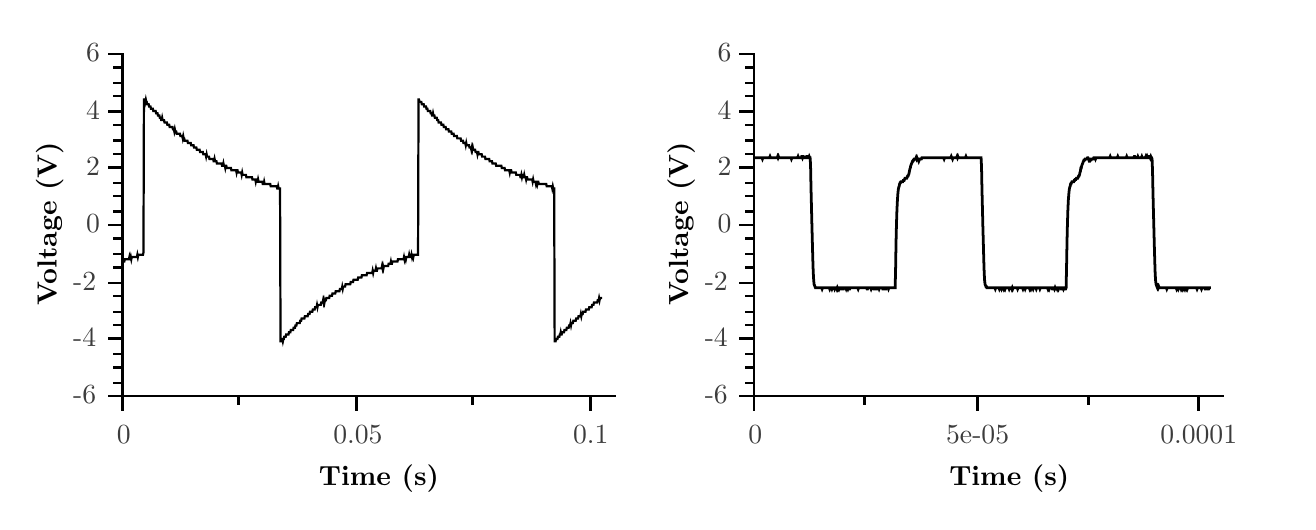
\begin{tikzpicture}{0pt}{0pt}{479pt}{180pt}
	\clip(0pt,180pt) -- (455.491pt,180pt) -- (455.491pt,8.83421pt) -- (0pt,8.83421pt) -- (0pt,180pt);
\begin{scope}
	\clip(262.454pt,170.491pt) -- (431.718pt,170.491pt) -- (431.718pt,46.8711pt) -- (262.454pt,46.8711pt) -- (262.454pt,170.491pt);
	\color[gray]{0}
	\draw[line width=1pt, line join=miter, line cap=rect](262.615pt,132.993pt) -- (262.776pt,132.993pt) -- (262.937pt,132.993pt) -- (263.098pt,132.993pt) -- (263.259pt,132.993pt) -- (263.42pt,132.993pt) -- (263.58pt,132.993pt) -- (263.741pt,132.993pt) -- (263.902pt,132.993pt) -- (264.063pt,132.993pt) -- (264.224pt,132.993pt) -- (264.385pt,132.993pt) -- (264.546pt,132.993pt) -- (264.707pt,132.993pt) -- (264.868pt,132.993pt) -- (265.029pt,132.993pt) -- (265.189pt,132.993pt) -- (265.35pt,132.993pt) -- (265.511pt,132.581pt) -- (265.672pt,132.993pt) -- (265.833pt,132.993pt) -- (265.994pt,132.993pt) -- (266.155pt,132.993pt) -- (266.316pt,132.993pt) -- (266.477pt,132.993pt) -- (266.638pt,132.993pt) -- (266.798pt,132.993pt) -- (266.959pt,132.993pt) -- (267.12pt,132.993pt) -- (267.281pt,132.993pt) -- (267.442pt,132.993pt) -- (267.603pt,132.993pt) -- (267.764pt,132.993pt) -- (267.925pt,132.993pt) -- (268.086pt,132.993pt) -- (268.247pt,133.405pt) -- (268.407pt,132.993pt) -- (268.568pt,132.993pt) -- (268.729pt,132.993pt) -- (268.89pt,132.993pt) -- (269.051pt,132.993pt) -- (269.212pt,132.993pt) -- (269.373pt,132.993pt) -- (269.534pt,132.993pt) -- (269.695pt,132.993pt) -- (269.855pt,132.993pt) -- (270.016pt,132.993pt) -- (270.177pt,132.993pt) -- (270.338pt,132.993pt) -- (270.499pt,132.993pt) -- (270.66pt,132.993pt) -- (270.821pt,132.993pt) -- (270.982pt,133.405pt) -- (271.143pt,132.993pt) -- (271.304pt,133.405pt) -- (271.464pt,132.993pt) -- (271.625pt,132.993pt) -- (271.786pt,132.993pt) -- (271.947pt,132.993pt) -- (272.108pt,132.993pt) -- (272.269pt,132.993pt) -- (272.43pt,132.993pt) -- (272.591pt,132.993pt) -- (272.752pt,132.993pt) -- (272.913pt,132.993pt) -- (273.073pt,132.993pt) -- (273.234pt,132.993pt) -- (273.395pt,132.993pt) -- (273.556pt,132.993pt) -- (273.717pt,132.993pt) -- (273.878pt,132.993pt) -- (274.039pt,132.993pt) -- (274.2pt,132.993pt) -- (274.361pt,132.993pt) -- (274.522pt,132.993pt) -- (274.682pt,132.993pt) -- (274.843pt,132.993pt) -- (275.004pt,132.993pt) -- (275.165pt,132.993pt) -- (275.326pt,132.993pt) -- (275.487pt,132.993pt) -- (275.648pt,132.993pt) -- (275.809pt,132.993pt) -- (275.97pt,132.581pt) -- (276.13pt,132.993pt) -- (276.291pt,132.993pt) -- (276.452pt,132.993pt) -- (276.613pt,132.993pt) -- (276.774pt,132.993pt) -- (276.935pt,132.993pt) -- (277.096pt,132.993pt) -- (277.257pt,132.993pt) -- (277.418pt,132.993pt) -- (277.579pt,132.993pt) -- (277.739pt,132.993pt) -- (277.9pt,132.993pt) -- (278.061pt,132.993pt) -- (278.222pt,132.993pt) -- (278.383pt,133.405pt) -- (278.544pt,132.993pt) -- (278.705pt,132.993pt) -- (278.866pt,132.993pt) -- (279.027pt,132.993pt) -- (279.188pt,132.993pt) -- (279.348pt,132.993pt) -- (279.509pt,132.993pt) -- (279.67pt,133.405pt) -- (279.831pt,133.405pt) -- (279.992pt,132.993pt) -- (280.153pt,133.405pt) -- (280.314pt,133.405pt) -- (280.475pt,132.993pt) -- (280.636pt,132.993pt) -- (280.797pt,132.993pt) -- (280.957pt,132.993pt) -- (281.118pt,132.993pt) -- (281.279pt,132.993pt) -- (281.44pt,133.405pt) -- (281.601pt,133.405pt) -- (281.762pt,133.405pt) -- (281.923pt,132.993pt) -- (282.084pt,132.993pt) -- (282.245pt,132.993pt) -- (282.405pt,133.405pt) -- (282.566pt,132.993pt) -- (282.727pt,132.993pt) -- (282.888pt,130.52pt) -- (283.049pt,122.279pt) -- (283.21pt,115.686pt) -- (283.371pt,109.093pt) -- (283.532pt,102.912pt) -- (283.693pt,96.731pt) -- (283.854pt,91.7862pt) -- (284.014pt,88.9018pt) -- (284.175pt,87.2535pt) -- (284.336pt,86.8414pt) -- (284.497pt,86.4294pt) -- (284.658pt,86.0173pt) -- (284.819pt,86.0173pt) -- (284.98pt,86.0173pt) -- (285.141pt,86.0173pt) -- (285.302pt,86.0173pt) -- (285.463pt,86.0173pt) -- (285.623pt,86.0173pt) -- (285.784pt,86.0173pt) -- (285.945pt,86.0173pt) -- (286.106pt,86.0173pt) -- (286.267pt,86.0173pt) -- (286.428pt,86.0173pt) -- (286.589pt,86.0173pt) -- (286.75pt,86.0173pt) -- (286.911pt,86.0173pt) -- (287.071pt,85.6052pt) -- (287.232pt,86.0173pt) -- (287.393pt,86.0173pt) -- (287.554pt,86.0173pt) -- (287.715pt,86.0173pt) -- (287.876pt,86.0173pt) -- (288.037pt,86.0173pt) -- (288.198pt,86.0173pt) -- (288.359pt,86.0173pt) -- (288.52pt,86.0173pt) -- (288.68pt,86.0173pt) -- (288.841pt,86.0173pt) -- (289.002pt,86.0173pt) -- (289.163pt,86.0173pt) -- (289.324pt,86.0173pt) -- (289.485pt,86.0173pt) -- (289.646pt,86.0173pt) -- (289.807pt,85.6052pt) -- (289.968pt,86.0173pt) -- (290.129pt,86.0173pt) -- (290.289pt,86.0173pt) -- (290.45pt,86.0173pt) -- (290.611pt,85.6052pt) -- (290.772pt,86.0173pt) -- (290.933pt,86.0173pt) -- (291.094pt,86.0173pt) -- (291.255pt,86.0173pt) -- (291.416pt,86.0173pt) -- (291.577pt,85.6052pt) -- (291.738pt,86.0173pt) -- (291.898pt,86.0173pt) -- (292.059pt,86.0173pt) -- (292.22pt,86.0173pt) -- (292.381pt,85.6052pt) -- (292.542pt,86.0173pt) -- (292.703pt,85.6052pt) -- (292.864pt,86.0173pt) -- (293.025pt,86.0173pt) -- (293.186pt,85.6052pt) -- (293.346pt,86.0173pt) -- (293.507pt,86.0173pt) -- (293.668pt,85.6052pt) -- (293.829pt,85.6052pt) -- (293.99pt,86.0173pt) -- (294.151pt,86.0173pt) -- (294.312pt,86.0173pt) -- (294.473pt,85.6052pt) -- (294.634pt,85.6052pt) -- (294.795pt,85.6052pt) -- (294.955pt,86.0173pt) -- (295.116pt,86.0173pt) -- (295.277pt,86.0173pt) -- (295.438pt,86.0173pt) -- (295.599pt,86.0173pt) -- (295.76pt,85.6052pt) -- (295.921pt,86.0173pt) -- (296.082pt,86.0173pt) -- (296.243pt,86.0173pt) -- (296.404pt,85.6052pt) -- (296.564pt,86.0173pt) -- (296.725pt,86.0173pt) -- (296.886pt,85.6052pt) -- (297.047pt,85.6052pt) -- (297.208pt,86.0173pt) -- (297.369pt,86.0173pt) -- (297.53pt,86.0173pt) -- (297.691pt,86.0173pt) -- (297.852pt,86.0173pt) -- (298.013pt,86.0173pt) -- (298.173pt,86.0173pt) -- (298.334pt,86.0173pt) -- (298.495pt,86.0173pt) -- (298.656pt,86.0173pt) -- (298.817pt,86.0173pt) -- (298.978pt,86.0173pt) -- (299.139pt,86.0173pt) -- (299.3pt,86.0173pt) -- (299.461pt,86.0173pt) -- (299.621pt,86.0173pt) -- (299.782pt,86.0173pt) -- (299.943pt,86.0173pt) -- (300.104pt,85.6052pt) -- (300.265pt,86.0173pt) -- (300.426pt,86.0173pt) -- (300.587pt,86.0173pt) -- (300.748pt,86.0173pt) -- (300.909pt,86.0173pt) -- (301.07pt,86.0173pt) -- (301.23pt,86.0173pt) -- (301.391pt,86.0173pt) -- (301.552pt,86.0173pt) -- (301.713pt,86.0173pt) -- (301.874pt,86.0173pt) -- (302.035pt,86.0173pt) -- (302.196pt,86.0173pt) -- (302.357pt,86.0173pt) -- (302.518pt,86.0173pt) -- (302.679pt,86.0173pt) -- (302.839pt,86.0173pt) -- (303pt,86.0173pt) -- (303.161pt,86.0173pt) -- (303.322pt,85.6052pt) -- (303.483pt,85.6052pt) -- (303.644pt,86.0173pt) -- (303.805pt,86.0173pt) -- (303.966pt,86.0173pt) -- (304.127pt,86.0173pt) -- (304.288pt,86.0173pt) -- (304.448pt,86.0173pt) -- (304.609pt,86.0173pt) -- (304.77pt,85.6052pt) -- (304.931pt,86.0173pt) -- (305.092pt,86.0173pt) -- (305.253pt,86.0173pt) -- (305.414pt,86.0173pt) -- (305.575pt,86.0173pt) -- (305.736pt,85.6052pt) -- (305.896pt,85.6052pt) -- (306.057pt,86.0173pt) -- (306.218pt,86.0173pt) -- (306.379pt,86.0173pt) -- (306.54pt,86.0173pt) -- (306.701pt,85.6052pt) -- (306.862pt,85.6052pt) -- (307.023pt,86.0173pt) -- (307.184pt,86.0173pt) -- (307.345pt,86.0173pt) -- (307.505pt,86.0173pt) -- (307.666pt,85.6052pt) -- (307.827pt,86.0173pt) -- (307.988pt,86.0173pt) -- (308.149pt,86.0173pt) -- (308.31pt,86.0173pt) -- (308.471pt,86.0173pt) -- (308.632pt,86.0173pt) -- (308.793pt,86.0173pt) -- (308.954pt,85.6052pt) -- (309.114pt,85.6052pt) -- (309.275pt,85.6052pt) -- (309.436pt,86.0173pt) -- (309.597pt,86.0173pt) -- (309.758pt,86.0173pt) -- (309.919pt,85.6052pt) -- (310.08pt,85.6052pt) -- (310.241pt,86.0173pt) -- (310.402pt,86.0173pt) -- (310.562pt,86.0173pt) -- (310.723pt,86.0173pt) -- (310.884pt,86.0173pt) -- (311.045pt,85.6052pt) -- (311.206pt,86.0173pt) -- (311.367pt,86.0173pt) -- (311.528pt,86.0173pt) -- (311.689pt,86.0173pt) -- (311.85pt,86.0173pt) -- (312.011pt,86.0173pt) -- (312.171pt,86.0173pt) -- (312.332pt,86.0173pt) -- (312.493pt,86.0173pt) -- (312.654pt,86.0173pt) -- (312.815pt,86.0173pt) -- (312.976pt,86.0173pt) -- (313.137pt,86.0173pt) -- (313.298pt,86.0173pt) -- (313.459pt,86.0173pt) -- (313.62pt,92.6104pt) -- (313.78pt,102.5pt) -- (313.941pt,109.093pt) -- (314.102pt,114.038pt) -- (314.263pt,117.334pt) -- (314.424pt,119.807pt) -- (314.585pt,121.455pt) -- (314.746pt,122.279pt) -- (314.907pt,122.691pt) -- (315.068pt,123.515pt) -- (315.229pt,123.927pt) -- (315.389pt,123.927pt) -- (315.55pt,124.339pt) -- (315.711pt,124.339pt) -- (315.872pt,124.339pt) -- (316.033pt,124.339pt) -- (316.194pt,124.339pt) -- (316.355pt,124.751pt) -- (316.516pt,124.751pt) -- (316.677pt,124.751pt) -- (316.837pt,125.164pt) -- (316.998pt,125.576pt) -- (317.159pt,125.576pt) -- (317.32pt,125.576pt) -- (317.481pt,125.576pt) -- (317.642pt,125.576pt) -- (317.803pt,125.988pt) -- (317.964pt,126.4pt) -- (318.125pt,126.4pt) -- (318.286pt,126.812pt) -- (318.446pt,127.224pt) -- (318.607pt,128.048pt) -- (318.768pt,128.872pt) -- (318.929pt,129.284pt) -- (319.09pt,130.108pt) -- (319.251pt,130.52pt) -- (319.412pt,130.932pt) -- (319.573pt,131.345pt) -- (319.734pt,131.757pt) -- (319.895pt,131.757pt) -- (320.055pt,132.169pt) -- (320.216pt,132.169pt) -- (320.377pt,132.581pt) -- (320.538pt,132.581pt) -- (320.699pt,132.581pt) -- (320.86pt,132.581pt) -- (321.021pt,132.993pt) -- (321.182pt,132.581pt) -- (321.343pt,132.993pt) -- (321.504pt,132.581pt) -- (321.664pt,132.581pt) -- (321.825pt,132.169pt) -- (321.986pt,131.757pt) -- (322.147pt,132.169pt) -- (322.308pt,132.581pt) -- (322.469pt,132.581pt) -- (322.63pt,132.581pt) -- (322.791pt,132.581pt) -- (322.952pt,132.581pt) -- (323.112pt,132.993pt) -- (323.273pt,132.993pt) -- (323.434pt,132.993pt) -- (323.595pt,132.993pt) -- (323.756pt,132.993pt) -- (323.917pt,132.993pt) -- (324.078pt,132.993pt) -- (324.239pt,132.993pt) -- (324.4pt,132.993pt) -- (324.561pt,132.993pt) -- (324.721pt,132.993pt) -- (324.882pt,132.993pt) -- (325.043pt,132.993pt) -- (325.204pt,132.993pt) -- (325.365pt,132.993pt) -- (325.526pt,132.993pt) -- (325.687pt,132.993pt) -- (325.848pt,132.993pt) -- (326.009pt,132.993pt) -- (326.17pt,132.993pt) -- (326.33pt,132.993pt) -- (326.491pt,132.993pt) -- (326.652pt,132.993pt) -- (326.813pt,132.993pt) -- (326.974pt,132.993pt) -- (327.135pt,132.993pt) -- (327.296pt,132.993pt) -- (327.457pt,132.993pt) -- (327.618pt,132.993pt) -- (327.779pt,132.993pt) -- (327.939pt,132.993pt) -- (328.1pt,132.993pt) -- (328.261pt,132.993pt) -- (328.422pt,132.993pt) -- (328.583pt,132.993pt) -- (328.744pt,132.993pt) -- (328.905pt,132.993pt) -- (329.066pt,132.993pt) -- (329.227pt,132.993pt) -- (329.387pt,132.993pt) -- (329.548pt,132.993pt) -- (329.709pt,132.993pt) -- (329.87pt,132.993pt) -- (330.031pt,132.993pt) -- (330.192pt,132.993pt) -- (330.353pt,132.993pt) -- (330.514pt,132.993pt) -- (330.675pt,132.993pt) -- (330.836pt,132.993pt) -- (330.996pt,132.993pt) -- (331.157pt,132.581pt) -- (331.318pt,132.993pt) -- (331.479pt,132.993pt) -- (331.64pt,132.993pt) -- (331.801pt,132.993pt) -- (331.962pt,132.993pt) -- (332.123pt,132.993pt) -- (332.284pt,132.993pt) -- (332.445pt,132.993pt) -- (332.605pt,132.993pt) -- (332.766pt,132.993pt) -- (332.927pt,132.993pt) -- (333.088pt,132.993pt) -- (333.249pt,132.993pt) -- (333.41pt,132.993pt) -- (333.571pt,132.993pt) -- (333.732pt,133.405pt) -- (333.893pt,132.993pt) -- (334.054pt,132.993pt) -- (334.214pt,132.581pt) -- (334.375pt,132.993pt) -- (334.536pt,132.993pt) -- (334.697pt,132.993pt) -- (334.858pt,132.993pt) -- (335.019pt,132.993pt) -- (335.18pt,132.993pt) -- (335.341pt,132.993pt) -- (335.502pt,132.993pt) -- (335.662pt,132.993pt) -- (335.823pt,133.405pt) -- (335.984pt,132.993pt) -- (336.145pt,133.405pt) -- (336.306pt,132.993pt) -- (336.467pt,132.993pt) -- (336.628pt,132.993pt) -- (336.789pt,132.993pt) -- (336.95pt,132.993pt) -- (337.111pt,132.993pt) -- (337.271pt,132.993pt) -- (337.432pt,132.993pt) -- (337.593pt,132.993pt) -- (337.754pt,132.993pt) -- (337.915pt,132.993pt) -- (338.076pt,132.993pt) -- (338.237pt,132.993pt) -- (338.398pt,132.993pt) -- (338.559pt,132.993pt) -- (338.72pt,132.993pt) -- (338.88pt,132.993pt) -- (339.041pt,133.405pt) -- (339.202pt,132.993pt) -- (339.363pt,132.993pt) -- (339.524pt,132.993pt) -- (339.685pt,132.993pt) -- (339.846pt,132.993pt) -- (340.007pt,132.993pt) -- (340.168pt,132.993pt) -- (340.328pt,132.993pt) -- (340.489pt,132.993pt) -- (340.65pt,132.993pt) -- (340.811pt,132.993pt) -- (340.972pt,132.993pt) -- (341.133pt,132.993pt) -- (341.294pt,132.993pt) -- (341.455pt,132.993pt) -- (341.616pt,132.993pt) -- (341.777pt,132.993pt) -- (341.937pt,132.993pt) -- (342.098pt,132.993pt) -- (342.259pt,132.993pt) -- (342.42pt,132.993pt) -- (342.581pt,132.993pt) -- (342.742pt,132.993pt) -- (342.903pt,132.993pt) -- (343.064pt,132.993pt) -- (343.225pt,132.993pt) -- (343.386pt,132.993pt) -- (343.546pt,132.993pt) -- (343.707pt,132.993pt) -- (343.868pt,132.993pt) -- (344.029pt,132.993pt) -- (344.19pt,132.993pt) -- (344.351pt,132.993pt) -- (344.512pt,132.993pt) -- (344.673pt,129.696pt) -- (344.834pt,121.455pt) -- (344.995pt,114.862pt) -- (345.155pt,108.269pt) -- (345.316pt,102.5pt) -- (345.477pt,96.3189pt) -- (345.638pt,91.3742pt) -- (345.799pt,88.4897pt) -- (345.96pt,87.2535pt) -- (346.121pt,86.8414pt) -- (346.282pt,86.4294pt) -- (346.443pt,86.4294pt) -- (346.603pt,86.0173pt) -- (346.764pt,86.0173pt) -- (346.925pt,86.0173pt) -- (347.086pt,86.0173pt) -- (347.247pt,86.0173pt) -- (347.408pt,86.0173pt) -- (347.569pt,86.0173pt) -- (347.73pt,86.0173pt) -- (347.891pt,86.0173pt) -- (348.052pt,86.0173pt) -- (348.212pt,86.0173pt) -- (348.373pt,86.0173pt) -- (348.534pt,86.0173pt) -- (348.695pt,86.0173pt) -- (348.856pt,86.0173pt) -- (349.017pt,86.0173pt) -- (349.178pt,86.0173pt) -- (349.339pt,86.0173pt) -- (349.5pt,86.0173pt) -- (349.661pt,85.6052pt) -- (349.821pt,86.0173pt) -- (349.982pt,86.0173pt) -- (350.143pt,86.0173pt) -- (350.304pt,86.0173pt) -- (350.465pt,86.0173pt) -- (350.626pt,86.0173pt) -- (350.787pt,86.0173pt) -- (350.948pt,86.0173pt) -- (351.109pt,85.6052pt) -- (351.27pt,86.0173pt) -- (351.43pt,86.0173pt) -- (351.591pt,86.0173pt) -- (351.752pt,86.0173pt) -- (351.913pt,85.6052pt) -- (352.074pt,86.0173pt) -- (352.235pt,86.0173pt) -- (352.396pt,86.0173pt) -- (352.557pt,86.0173pt) -- (352.718pt,85.6052pt) -- (352.878pt,86.0173pt) -- (353.039pt,86.0173pt) -- (353.2pt,85.6052pt) -- (353.361pt,86.0173pt) -- (353.522pt,86.0173pt) -- (353.683pt,86.0173pt) -- (353.844pt,86.0173pt) -- (354.005pt,86.0173pt) -- (354.166pt,86.0173pt) -- (354.327pt,86.0173pt) -- (354.487pt,86.0173pt) -- (354.648pt,85.6052pt) -- (354.809pt,86.0173pt) -- (354.97pt,86.0173pt) -- (355.131pt,86.0173pt) -- (355.292pt,86.0173pt) -- (355.453pt,86.0173pt) -- (355.614pt,85.6052pt) -- (355.775pt,86.0173pt) -- (355.936pt,85.6052pt) -- (356.096pt,86.0173pt) -- (356.257pt,86.0173pt) -- (356.418pt,86.0173pt) -- (356.579pt,86.0173pt) -- (356.74pt,86.0173pt) -- (356.901pt,86.0173pt) -- (357.062pt,86.0173pt) -- (357.223pt,86.0173pt) -- (357.384pt,86.0173pt) -- (357.545pt,86.0173pt) -- (357.705pt,85.6052pt) -- (357.866pt,86.0173pt) -- (358.027pt,86.0173pt) -- (358.188pt,86.0173pt) -- (358.349pt,86.0173pt) -- (358.51pt,86.0173pt) -- (358.671pt,86.0173pt) -- (358.832pt,86.0173pt) -- (358.993pt,86.0173pt) -- (359.153pt,86.0173pt) -- (359.314pt,86.0173pt) -- (359.475pt,86.0173pt) -- (359.636pt,85.6052pt) -- (359.797pt,86.0173pt) -- (359.958pt,86.0173pt) -- (360.119pt,86.0173pt) -- (360.28pt,86.0173pt) -- (360.441pt,85.6052pt) -- (360.602pt,86.0173pt) -- (360.762pt,86.0173pt) -- (360.923pt,86.0173pt) -- (361.084pt,86.0173pt) -- (361.245pt,86.0173pt) -- (361.406pt,86.0173pt) -- (361.567pt,86.0173pt) -- (361.728pt,86.0173pt) -- (361.889pt,86.0173pt) -- (362.05pt,85.6052pt) -- (362.211pt,86.0173pt) -- (362.371pt,86.0173pt) -- (362.532pt,85.6052pt) -- (362.693pt,86.0173pt) -- (362.854pt,86.0173pt) -- (363.015pt,86.0173pt) -- (363.176pt,86.0173pt) -- (363.337pt,85.6052pt) -- (363.498pt,86.0173pt) -- (363.659pt,86.0173pt) -- (363.82pt,86.0173pt) -- (363.98pt,86.0173pt) -- (364.141pt,86.0173pt) -- (364.302pt,86.0173pt) -- (364.463pt,85.6052pt) -- (364.624pt,86.0173pt) -- (364.785pt,86.0173pt) -- (364.946pt,86.0173pt) -- (365.107pt,86.0173pt) -- (365.268pt,86.0173pt) -- (365.428pt,86.0173pt) -- (365.589pt,86.0173pt) -- (365.75pt,85.6052pt) -- (365.911pt,86.0173pt) -- (366.072pt,86.0173pt) -- (366.233pt,86.0173pt) -- (366.394pt,86.0173pt) -- (366.555pt,86.0173pt) -- (366.716pt,86.0173pt) -- (366.877pt,86.0173pt) -- (367.037pt,86.0173pt) -- (367.198pt,86.0173pt) -- (367.359pt,86.0173pt) -- (367.52pt,86.0173pt) -- (367.681pt,86.0173pt) -- (367.842pt,86.0173pt) -- (368.003pt,86.0173pt) -- (368.164pt,86.0173pt) -- (368.325pt,86.0173pt) -- (368.486pt,86.0173pt) -- (368.646pt,85.6052pt) -- (368.807pt,86.0173pt) -- (368.968pt,86.0173pt) -- (369.129pt,85.6052pt) -- (369.29pt,86.0173pt) -- (369.451pt,86.0173pt) -- (369.612pt,86.0173pt) -- (369.773pt,86.0173pt) -- (369.934pt,86.0173pt) -- (370.094pt,86.0173pt) -- (370.255pt,85.6052pt) -- (370.416pt,85.6052pt) -- (370.577pt,86.0173pt) -- (370.738pt,86.0173pt) -- (370.899pt,86.0173pt) -- (371.06pt,85.6052pt) -- (371.221pt,86.0173pt) -- (371.382pt,85.6052pt) -- (371.543pt,85.6052pt) -- (371.703pt,86.0173pt) -- (371.864pt,86.0173pt) -- (372.025pt,85.6052pt) -- (372.186pt,86.0173pt) -- (372.347pt,86.0173pt) -- (372.508pt,85.6052pt) -- (372.669pt,86.0173pt) -- (372.83pt,86.0173pt) -- (372.991pt,86.0173pt) -- (373.152pt,86.0173pt) -- (373.312pt,86.0173pt) -- (373.473pt,85.6052pt) -- (373.634pt,85.6052pt) -- (373.795pt,86.0173pt) -- (373.956pt,86.0173pt) -- (374.117pt,86.0173pt) -- (374.278pt,85.6052pt) -- (374.439pt,86.0173pt) -- (374.6pt,86.0173pt) -- (374.761pt,86.0173pt) -- (374.921pt,85.6052pt) -- (375.082pt,85.6052pt) -- (375.243pt,86.0173pt) -- (375.404pt,93.8466pt) -- (375.565pt,102.912pt) -- (375.726pt,109.505pt) -- (375.887pt,114.45pt) -- (376.048pt,117.746pt) -- (376.209pt,119.807pt) -- (376.369pt,121.455pt) -- (376.53pt,122.279pt) -- (376.691pt,122.691pt) -- (376.852pt,123.515pt) -- (377.013pt,123.515pt) -- (377.174pt,123.927pt) -- (377.335pt,124.339pt) -- (377.496pt,124.339pt) -- (377.657pt,124.339pt) -- (377.818pt,124.339pt) -- (377.978pt,124.339pt) -- (378.139pt,124.751pt) -- (378.3pt,124.751pt) -- (378.461pt,125.164pt) -- (378.622pt,125.164pt) -- (378.783pt,125.164pt) -- (378.944pt,125.576pt) -- (379.105pt,125.576pt) -- (379.266pt,125.576pt) -- (379.427pt,125.576pt) -- (379.587pt,125.988pt) -- (379.748pt,126.4pt) -- (379.909pt,126.4pt) -- (380.07pt,126.812pt) -- (380.231pt,127.636pt) -- (380.392pt,128.048pt) -- (380.553pt,129.284pt) -- (380.714pt,129.284pt) -- (380.875pt,130.108pt) -- (381.036pt,130.52pt) -- (381.196pt,130.932pt) -- (381.357pt,131.345pt) -- (381.518pt,131.757pt) -- (381.679pt,132.169pt) -- (381.84pt,132.169pt) -- (382.001pt,132.169pt) -- (382.162pt,132.581pt) -- (382.323pt,132.581pt) -- (382.484pt,132.581pt) -- (382.644pt,132.581pt) -- (382.805pt,132.581pt) -- (382.966pt,132.993pt) -- (383.127pt,132.993pt) -- (383.288pt,132.581pt) -- (383.449pt,132.581pt) -- (383.61pt,131.757pt) -- (383.771pt,131.757pt) -- (383.932pt,132.169pt) -- (384.093pt,132.169pt) -- (384.253pt,132.169pt) -- (384.414pt,132.581pt) -- (384.575pt,132.581pt) -- (384.736pt,132.581pt) -- (384.897pt,132.581pt) -- (385.058pt,132.581pt) -- (385.219pt,132.993pt) -- (385.38pt,132.993pt) -- (385.541pt,132.993pt) -- (385.702pt,132.993pt) -- (385.862pt,132.581pt) -- (386.023pt,132.993pt) -- (386.184pt,132.993pt) -- (386.345pt,132.993pt) -- (386.506pt,132.993pt) -- (386.667pt,132.993pt) -- (386.828pt,132.993pt) -- (386.989pt,132.993pt) -- (387.15pt,132.993pt) -- (387.311pt,132.993pt) -- (387.471pt,132.993pt) -- (387.632pt,132.993pt) -- (387.793pt,132.993pt) -- (387.954pt,132.993pt) -- (388.115pt,132.993pt) -- (388.276pt,132.993pt) -- (388.437pt,132.993pt) -- (388.598pt,132.993pt) -- (388.759pt,132.993pt) -- (388.919pt,132.993pt) -- (389.08pt,132.993pt) -- (389.241pt,132.993pt) -- (389.402pt,132.993pt) -- (389.563pt,132.993pt) -- (389.724pt,132.993pt) -- (389.885pt,132.993pt) -- (390.046pt,132.993pt) -- (390.207pt,132.993pt) -- (390.368pt,132.993pt) -- (390.528pt,132.993pt) -- (390.689pt,132.993pt) -- (390.85pt,132.993pt) -- (391.011pt,132.993pt) -- (391.172pt,133.405pt) -- (391.333pt,132.993pt) -- (391.494pt,132.993pt) -- (391.655pt,132.993pt) -- (391.816pt,132.993pt) -- (391.977pt,132.993pt) -- (392.137pt,132.993pt) -- (392.298pt,132.993pt) -- (392.459pt,132.993pt) -- (392.62pt,132.993pt) -- (392.781pt,132.993pt) -- (392.942pt,132.993pt) -- (393.103pt,132.993pt) -- (393.264pt,132.993pt) -- (393.425pt,132.993pt) -- (393.586pt,132.993pt) -- (393.746pt,132.993pt) -- (393.907pt,133.405pt) -- (394.068pt,132.993pt) -- (394.229pt,132.993pt) -- (394.39pt,132.993pt) -- (394.551pt,132.993pt) -- (394.712pt,132.993pt) -- (394.873pt,132.993pt) -- (395.034pt,132.993pt) -- (395.194pt,132.993pt) -- (395.355pt,132.993pt) -- (395.516pt,132.993pt) -- (395.677pt,132.993pt) -- (395.838pt,132.993pt) -- (395.999pt,132.993pt) -- (396.16pt,132.993pt) -- (396.321pt,132.993pt) -- (396.482pt,132.993pt) -- (396.643pt,132.993pt) -- (396.803pt,132.993pt) -- (396.964pt,132.993pt) -- (397.125pt,133.405pt) -- (397.286pt,132.993pt) -- (397.447pt,132.993pt) -- (397.608pt,132.993pt) -- (397.769pt,132.993pt) -- (397.93pt,132.993pt) -- (398.091pt,132.993pt) -- (398.252pt,132.993pt) -- (398.412pt,132.993pt) -- (398.573pt,132.993pt) -- (398.734pt,132.993pt) -- (398.895pt,132.993pt) -- (399.056pt,132.993pt) -- (399.217pt,132.993pt) -- (399.378pt,132.993pt) -- (399.539pt,132.993pt) -- (399.7pt,132.993pt) -- (399.86pt,133.405pt) -- (400.021pt,133.405pt) -- (400.182pt,132.993pt) -- (400.343pt,132.993pt) -- (400.504pt,132.993pt) -- (400.665pt,132.993pt) -- (400.826pt,132.993pt) -- (400.987pt,132.993pt) -- (401.148pt,133.405pt) -- (401.309pt,132.993pt) -- (401.469pt,132.993pt) -- (401.63pt,132.993pt) -- (401.791pt,132.993pt) -- (401.952pt,132.993pt) -- (402.113pt,132.993pt) -- (402.274pt,132.993pt) -- (402.435pt,132.993pt) -- (402.596pt,133.405pt) -- (402.757pt,132.993pt) -- (402.918pt,132.993pt) -- (403.078pt,132.993pt) -- (403.239pt,132.993pt) -- (403.4pt,132.993pt) -- (403.561pt,132.993pt) -- (403.722pt,132.993pt) -- (403.883pt,132.993pt) -- (404.044pt,133.405pt) -- (404.205pt,132.993pt) -- (404.366pt,132.993pt) -- (404.527pt,133.405pt) -- (404.687pt,132.993pt) -- (404.848pt,132.993pt) -- (405.009pt,132.993pt) -- (405.17pt,133.405pt) -- (405.331pt,133.405pt) -- (405.492pt,133.405pt) -- (405.653pt,132.993pt) -- (405.814pt,133.405pt) -- (405.975pt,132.993pt) -- (406.135pt,132.993pt) -- (406.296pt,132.581pt) -- (406.457pt,128.46pt) -- (406.618pt,120.631pt) -- (406.779pt,114.038pt) -- (406.94pt,107.857pt) -- (407.101pt,101.676pt) -- (407.262pt,95.9069pt) -- (407.423pt,90.9621pt) -- (407.584pt,88.4897pt) -- (407.744pt,87.2535pt) -- (407.905pt,86.8414pt) -- (408.066pt,86.4294pt) -- (408.227pt,86.0173pt) -- (408.388pt,86.4294pt) -- (408.549pt,86.0173pt) -- (408.71pt,86.4294pt) -- (408.871pt,86.0173pt) -- (409.032pt,86.0173pt) -- (409.193pt,86.0173pt) -- (409.353pt,86.0173pt) -- (409.514pt,86.0173pt) -- (409.675pt,86.0173pt) -- (409.836pt,86.0173pt) -- (409.997pt,86.0173pt) -- (410.158pt,86.0173pt) -- (410.319pt,86.0173pt) -- (410.48pt,86.0173pt) -- (410.641pt,86.0173pt) -- (410.802pt,86.0173pt) -- (410.962pt,86.0173pt) -- (411.123pt,86.0173pt) -- (411.284pt,86.0173pt) -- (411.445pt,86.0173pt) -- (411.606pt,85.6052pt) -- (411.767pt,86.0173pt) -- (411.928pt,86.0173pt) -- (412.089pt,86.0173pt) -- (412.25pt,86.0173pt) -- (412.41pt,86.0173pt) -- (412.571pt,86.0173pt) -- (412.732pt,86.0173pt) -- (412.893pt,86.0173pt) -- (413.054pt,86.0173pt) -- (413.215pt,86.0173pt) -- (413.376pt,86.0173pt) -- (413.537pt,86.0173pt) -- (413.698pt,86.0173pt) -- (413.859pt,86.0173pt) -- (414.019pt,86.0173pt) -- (414.18pt,86.0173pt) -- (414.341pt,86.0173pt) -- (414.502pt,86.0173pt) -- (414.663pt,86.0173pt) -- (414.824pt,86.0173pt) -- (414.985pt,86.0173pt) -- (415.146pt,85.6052pt) -- (415.307pt,86.0173pt) -- (415.468pt,86.0173pt) -- (415.628pt,86.0173pt) -- (415.789pt,85.6052pt) -- (415.95pt,86.0173pt) -- (416.111pt,86.0173pt) -- (416.272pt,86.0173pt) -- (416.433pt,86.0173pt) -- (416.594pt,86.0173pt) -- (416.755pt,85.6052pt) -- (416.916pt,86.0173pt) -- (417.077pt,86.0173pt) -- (417.237pt,85.6052pt) -- (417.398pt,86.0173pt) -- (417.559pt,86.0173pt) -- (417.72pt,86.0173pt) -- (417.881pt,85.6052pt) -- (418.042pt,86.0173pt) -- (418.203pt,86.0173pt) -- (418.364pt,86.0173pt) -- (418.525pt,85.6052pt) -- (418.685pt,86.0173pt) -- (418.846pt,86.0173pt) -- (419.007pt,85.6052pt) -- (419.168pt,86.0173pt) -- (419.329pt,86.0173pt) -- (419.49pt,86.0173pt) -- (419.651pt,86.0173pt) -- (419.812pt,86.0173pt) -- (419.973pt,86.0173pt) -- (420.134pt,86.0173pt) -- (420.294pt,86.0173pt) -- (420.455pt,86.0173pt) -- (420.616pt,86.0173pt) -- (420.777pt,86.0173pt) -- (420.938pt,86.0173pt) -- (421.099pt,86.0173pt) -- (421.26pt,86.0173pt) -- (421.421pt,86.0173pt) -- (421.582pt,86.0173pt) -- (421.743pt,86.0173pt) -- (421.903pt,86.0173pt) -- (422.064pt,86.0173pt) -- (422.225pt,86.0173pt) -- (422.386pt,86.0173pt) -- (422.547pt,85.6052pt) -- (422.708pt,86.0173pt) -- (422.869pt,86.0173pt) -- (423.03pt,86.0173pt) -- (423.191pt,86.0173pt) -- (423.351pt,86.0173pt) -- (423.512pt,86.0173pt) -- (423.673pt,86.0173pt) -- (423.834pt,86.0173pt) -- (423.995pt,86.0173pt) -- (424.156pt,85.6052pt) -- (424.317pt,86.0173pt) -- (424.478pt,86.0173pt) -- (424.639pt,86.0173pt) -- (424.8pt,86.0173pt) -- (424.96pt,86.0173pt) -- (425.121pt,86.0173pt) -- (425.282pt,86.0173pt) -- (425.443pt,85.6052pt) -- (425.604pt,85.6052pt) -- (425.765pt,86.0173pt) -- (425.926pt,86.0173pt) -- (426.087pt,86.0173pt) -- (426.248pt,86.0173pt) -- (426.409pt,85.6052pt) -- (426.569pt,85.6052pt) -- (426.73pt,85.6052pt) -- (426.891pt,86.0173pt) -- (427.052pt,86.0173pt);
\end{scope}
\begin{scope}
	\color[gray]{0}
	\pgftext[center, base, at={\pgfpoint{238.681pt}{109.156pt}},rotate=90]{\textbf{Voltage (V)}}
	\color[gray]{0.235294}
	\pgftext[center, base, at={\pgfpoint{248.829pt}{44.0183pt}}]{-6}
	\pgftext[center, base, at={\pgfpoint{248.829pt}{64.9386pt}}]{-4}
	\pgftext[center, base, at={\pgfpoint{248.829pt}{84.9079pt}}]{-2}
	\pgftext[center, base, at={\pgfpoint{251.838pt}{105.828pt}}]{0}
	\pgftext[center, base, at={\pgfpoint{251.838pt}{126.748pt}}]{2}
	\pgftext[center, base, at={\pgfpoint{251.838pt}{146.718pt}}]{4}
	\pgftext[center, base, at={\pgfpoint{251.838pt}{167.638pt}}]{6}
	\color[gray]{0}
	\draw[line width=1pt, line join=bevel, line cap=rect](262.454pt,51.6257pt) -- (259.601pt,51.6257pt);
	\draw[line width=1pt, line join=bevel, line cap=rect](262.454pt,62.0858pt) -- (259.601pt,62.0858pt);
	\draw[line width=1pt, line join=bevel, line cap=rect](262.454pt,72.5459pt) -- (259.601pt,72.5459pt);
	\draw[line width=1pt, line join=bevel, line cap=rect](262.454pt,83.0061pt) -- (259.601pt,83.0061pt);
	\draw[line width=1pt, line join=bevel, line cap=rect](262.454pt,93.4662pt) -- (259.601pt,93.4662pt);
	\draw[line width=1pt, line join=bevel, line cap=rect](262.454pt,103.926pt) -- (259.601pt,103.926pt);
	\draw[line width=1pt, line join=bevel, line cap=rect](262.454pt,113.436pt) -- (259.601pt,113.436pt);
	\draw[line width=1pt, line join=bevel, line cap=rect](262.454pt,123.896pt) -- (259.601pt,123.896pt);
	\draw[line width=1pt, line join=bevel, line cap=rect](262.454pt,134.356pt) -- (259.601pt,134.356pt);
	\draw[line width=1pt, line join=bevel, line cap=rect](262.454pt,144.816pt) -- (259.601pt,144.816pt);
	\draw[line width=1pt, line join=bevel, line cap=rect](262.454pt,155.276pt) -- (259.601pt,155.276pt);
	\draw[line width=1pt, line join=bevel, line cap=rect](262.454pt,165.736pt) -- (259.601pt,165.736pt);
	\draw[line width=1pt, line join=bevel, line cap=rect](262.454pt,57.3312pt) -- (259.601pt,57.3312pt);
	\draw[line width=1pt, line join=bevel, line cap=rect](262.454pt,77.3005pt) -- (259.601pt,77.3005pt);
	\draw[line width=1pt, line join=bevel, line cap=rect](262.454pt,98.2208pt) -- (259.601pt,98.2208pt);
	\draw[line width=1pt, line join=bevel, line cap=rect](262.454pt,119.141pt) -- (259.601pt,119.141pt);
	\draw[line width=1pt, line join=bevel, line cap=rect](262.454pt,139.11pt) -- (259.601pt,139.11pt);
	\draw[line width=1pt, line join=bevel, line cap=rect](262.454pt,160.031pt) -- (259.601pt,160.031pt);
	\draw[line width=1pt, line join=bevel, line cap=rect](262.454pt,46.8711pt) -- (257.7pt,46.8711pt);
	\draw[line width=1pt, line join=bevel, line cap=rect](262.454pt,67.7913pt) -- (257.7pt,67.7913pt);
	\draw[line width=1pt, line join=bevel, line cap=rect](262.454pt,87.7607pt) -- (257.7pt,87.7607pt);
	\draw[line width=1pt, line join=bevel, line cap=rect](262.454pt,108.681pt) -- (257.7pt,108.681pt);
	\draw[line width=1pt, line join=bevel, line cap=rect](262.454pt,129.601pt) -- (257.7pt,129.601pt);
	\draw[line width=1pt, line join=bevel, line cap=rect](262.454pt,149.571pt) -- (257.7pt,149.571pt);
	\draw[line width=1pt, line join=bevel, line cap=rect](262.454pt,170.491pt) -- (257.7pt,170.491pt);
	\draw[line width=1pt, line join=bevel, line cap=rect](262.454pt,170.491pt) -- (262.454pt,46.8711pt);
	\pgftext[center, base, at={\pgfpoint{354.694pt}{14.5397pt}}]{\textbf{Time (s)}}
	\color[gray]{0.235294}
	\pgftext[center, base, at={\pgfpoint{262.922pt}{29.7545pt}}]{0}
	\pgftext[center, base, at={\pgfpoint{343.275pt}{29.7545pt}}]{5e-05}
	\pgftext[center, base, at={\pgfpoint{423.152pt}{29.7545pt}}]{0.0001}
	\color[gray]{0}
	\draw[line width=1pt, line join=bevel, line cap=rect](302.393pt,46.8711pt) -- (302.393pt,44.0183pt);
	\draw[line width=1pt, line join=bevel, line cap=rect](383.221pt,46.8711pt) -- (383.221pt,44.0183pt);
	\draw[line width=1pt, line join=bevel, line cap=rect](262.454pt,46.8711pt) -- (262.454pt,42.1164pt);
	\draw[line width=1pt, line join=bevel, line cap=rect](343.282pt,46.8711pt) -- (343.282pt,42.1164pt);
	\draw[line width=1pt, line join=bevel, line cap=rect](423.16pt,46.8711pt) -- (423.16pt,42.1164pt);
	\draw[line width=1pt, line join=bevel, line cap=rect](262.454pt,46.8711pt) -- (431.718pt,46.8711pt);
\end{scope}
\begin{scope}
	\clip(34.2332pt,170.491pt) -- (212.055pt,170.491pt) -- (212.055pt,46.8711pt) -- (34.2332pt,46.8711pt) -- (34.2332pt,170.491pt);
	\color[gray]{0}
	\draw[line width=0.8pt, line join=miter, line cap=rect](34.4022pt,95.4948pt) -- (34.5712pt,95.4948pt) -- (34.7403pt,95.4948pt) -- (34.9093pt,95.4948pt) -- (35.0783pt,96.3189pt) -- (35.2474pt,96.3189pt) -- (35.4164pt,96.3189pt) -- (35.5854pt,96.3189pt) -- (35.7545pt,96.3189pt) -- (35.9235pt,96.3189pt) -- (36.0925pt,96.3189pt) -- (36.2615pt,96.3189pt) -- (36.4306pt,96.3189pt) -- (36.5996pt,96.3189pt) -- (36.7686pt,97.1431pt) -- (36.9377pt,96.3189pt) -- (37.1067pt,96.3189pt) -- (37.2757pt,97.1431pt) -- (37.4448pt,96.3189pt) -- (37.6138pt,97.1431pt) -- (37.7828pt,97.1431pt) -- (37.9519pt,97.1431pt) -- (38.1209pt,97.1431pt) -- (38.2899pt,97.1431pt) -- (38.459pt,97.1431pt) -- (38.628pt,97.1431pt) -- (38.797pt,97.1431pt) -- (38.9661pt,97.1431pt) -- (39.1351pt,97.1431pt) -- (39.3041pt,97.1431pt) -- (39.4732pt,97.1431pt) -- (39.6422pt,97.9672pt) -- (39.8112pt,97.1431pt) -- (39.9803pt,97.9672pt) -- (40.1493pt,97.9672pt) -- (40.3183pt,97.9672pt) -- (40.4874pt,97.9672pt) -- (40.6564pt,97.9672pt) -- (40.8254pt,97.9672pt) -- (40.9945pt,97.9672pt) -- (41.1635pt,97.9672pt) -- (41.3325pt,97.9672pt) -- (41.5016pt,97.9672pt) -- (41.6706pt,97.9672pt) -- (41.8396pt,98.7913pt) -- (42.0087pt,154.008pt) -- (42.1777pt,154.008pt) -- (42.3467pt,154.008pt) -- (42.5158pt,153.184pt) -- (42.6848pt,154.008pt) -- (42.8538pt,153.184pt) -- (43.0229pt,153.184pt) -- (43.1919pt,152.36pt) -- (43.3609pt,152.36pt) -- (43.5299pt,152.36pt) -- (43.699pt,152.36pt) -- (43.868pt,151.536pt) -- (44.037pt,151.536pt) -- (44.2061pt,151.536pt) -- (44.3751pt,151.536pt) -- (44.5441pt,150.712pt) -- (44.7132pt,150.712pt) -- (44.8822pt,150.712pt) -- (45.0512pt,150.712pt) -- (45.2203pt,150.712pt) -- (45.3893pt,149.887pt) -- (45.5583pt,149.887pt) -- (45.7274pt,149.887pt) -- (45.8964pt,149.887pt) -- (46.0654pt,149.887pt) -- (46.2345pt,149.887pt) -- (46.4035pt,149.063pt) -- (46.5725pt,149.063pt) -- (46.7416pt,149.063pt) -- (46.9106pt,149.063pt) -- (47.0796pt,148.239pt) -- (47.2487pt,148.239pt) -- (47.4177pt,148.239pt) -- (47.5867pt,148.239pt) -- (47.7558pt,147.415pt) -- (47.9248pt,147.415pt) -- (48.0938pt,147.415pt) -- (48.2629pt,146.591pt) -- (48.4319pt,146.591pt) -- (48.6009pt,147.415pt) -- (48.77pt,146.591pt) -- (48.939pt,146.591pt) -- (49.108pt,146.591pt) -- (49.2771pt,146.591pt) -- (49.4461pt,145.767pt) -- (49.6151pt,145.767pt) -- (49.7842pt,145.767pt) -- (49.9532pt,145.767pt) -- (50.1222pt,145.767pt) -- (50.2912pt,145.767pt) -- (50.4603pt,144.943pt) -- (50.6293pt,144.943pt) -- (50.7983pt,144.943pt) -- (50.9674pt,144.943pt) -- (51.1364pt,144.943pt) -- (51.3054pt,144.119pt) -- (51.4745pt,144.119pt) -- (51.6435pt,144.119pt) -- (51.8125pt,144.119pt) -- (51.9816pt,144.119pt) -- (52.1506pt,144.119pt) -- (52.3196pt,144.119pt) -- (52.4887pt,143.294pt) -- (52.6577pt,143.294pt) -- (52.8267pt,143.294pt) -- (52.9958pt,142.47pt) -- (53.1648pt,143.294pt) -- (53.3338pt,142.47pt) -- (53.5029pt,142.47pt) -- (53.6719pt,142.47pt) -- (53.8409pt,141.646pt) -- (54.01pt,141.646pt) -- (54.179pt,141.646pt) -- (54.348pt,141.646pt) -- (54.5171pt,141.646pt) -- (54.6861pt,141.646pt) -- (54.8551pt,141.646pt) -- (55.0242pt,141.646pt) -- (55.1932pt,140.822pt) -- (55.3622pt,140.822pt) -- (55.5313pt,140.822pt) -- (55.7003pt,140.822pt) -- (55.8693pt,140.822pt) -- (56.0384pt,139.998pt) -- (56.2074pt,140.822pt) -- (56.3764pt,139.998pt) -- (56.5455pt,139.998pt) -- (56.7145pt,139.174pt) -- (56.8835pt,139.174pt) -- (57.0526pt,139.174pt) -- (57.2216pt,139.174pt) -- (57.3906pt,139.174pt) -- (57.5596pt,139.174pt) -- (57.7287pt,139.174pt) -- (57.8977pt,138.35pt) -- (58.0667pt,138.35pt) -- (58.2358pt,138.35pt) -- (58.4048pt,138.35pt) -- (58.5738pt,138.35pt) -- (58.7429pt,138.35pt) -- (58.9119pt,138.35pt) -- (59.0809pt,137.526pt) -- (59.25pt,137.526pt) -- (59.419pt,137.526pt) -- (59.588pt,137.526pt) -- (59.7571pt,137.526pt) -- (59.9261pt,137.526pt) -- (60.0951pt,136.701pt) -- (60.2642pt,136.701pt) -- (60.4332pt,136.701pt) -- (60.6022pt,136.701pt) -- (60.7713pt,136.701pt) -- (60.9403pt,136.701pt) -- (61.1093pt,135.877pt) -- (61.2784pt,135.877pt) -- (61.4474pt,135.877pt) -- (61.6164pt,135.877pt) -- (61.7855pt,135.877pt) -- (61.9545pt,135.877pt) -- (62.1235pt,135.877pt) -- (62.2926pt,135.053pt) -- (62.4616pt,135.053pt) -- (62.6306pt,135.053pt) -- (62.7997pt,135.053pt) -- (62.9687pt,135.053pt) -- (63.1377pt,135.053pt) -- (63.3068pt,135.053pt) -- (63.4758pt,134.229pt) -- (63.6448pt,134.229pt) -- (63.8139pt,134.229pt) -- (63.9829pt,134.229pt) -- (64.1519pt,134.229pt) -- (64.321pt,134.229pt) -- (64.49pt,133.405pt) -- (64.659pt,134.229pt) -- (64.828pt,133.405pt) -- (64.9971pt,133.405pt) -- (65.1661pt,133.405pt) -- (65.3351pt,133.405pt) -- (65.5042pt,133.405pt) -- (65.6732pt,132.581pt) -- (65.8422pt,132.581pt) -- (66.0113pt,132.581pt) -- (66.1803pt,132.581pt) -- (66.3493pt,132.581pt) -- (66.5184pt,132.581pt) -- (66.6874pt,132.581pt) -- (66.8564pt,132.581pt) -- (67.0255pt,132.581pt) -- (67.1945pt,131.757pt) -- (67.3635pt,131.757pt) -- (67.5326pt,132.581pt) -- (67.7016pt,131.757pt) -- (67.8706pt,131.757pt) -- (68.0397pt,131.757pt) -- (68.2087pt,131.757pt) -- (68.3777pt,130.932pt) -- (68.5468pt,130.932pt) -- (68.7158pt,130.932pt) -- (68.8848pt,130.932pt) -- (69.0539pt,130.932pt) -- (69.2229pt,130.932pt) -- (69.3919pt,130.932pt) -- (69.561pt,130.932pt) -- (69.73pt,130.932pt) -- (69.899pt,130.932pt) -- (70.0681pt,130.932pt) -- (70.2371pt,130.108pt) -- (70.4061pt,130.108pt) -- (70.5752pt,130.108pt) -- (70.7442pt,130.932pt) -- (70.9132pt,130.108pt) -- (71.0823pt,130.108pt) -- (71.2513pt,130.108pt) -- (71.4203pt,129.284pt) -- (71.5894pt,130.108pt) -- (71.7584pt,130.108pt) -- (71.9274pt,129.284pt) -- (72.0964pt,129.284pt) -- (72.2655pt,129.284pt) -- (72.4345pt,129.284pt) -- (72.6035pt,129.284pt) -- (72.7726pt,129.284pt) -- (72.9416pt,129.284pt) -- (73.1106pt,129.284pt) -- (73.2797pt,129.284pt) -- (73.4487pt,129.284pt) -- (73.6177pt,128.46pt) -- (73.7868pt,128.46pt) -- (73.9558pt,128.46pt) -- (74.1248pt,128.46pt) -- (74.2939pt,128.46pt) -- (74.4629pt,128.46pt) -- (74.6319pt,128.46pt) -- (74.801pt,128.46pt) -- (74.97pt,128.46pt) -- (75.139pt,128.46pt) -- (75.3081pt,128.46pt) -- (75.4771pt,127.636pt) -- (75.6461pt,128.46pt) -- (75.8152pt,128.46pt) -- (75.9842pt,127.636pt) -- (76.1532pt,127.636pt) -- (76.3223pt,127.636pt) -- (76.4913pt,127.636pt) -- (76.6603pt,127.636pt) -- (76.8294pt,127.636pt) -- (76.9984pt,127.636pt) -- (77.1674pt,127.636pt) -- (77.3365pt,126.812pt) -- (77.5055pt,127.636pt) -- (77.6745pt,126.812pt) -- (77.8436pt,126.812pt) -- (78.0126pt,126.812pt) -- (78.1816pt,126.812pt) -- (78.3507pt,126.812pt) -- (78.5197pt,126.812pt) -- (78.6887pt,126.812pt) -- (78.8577pt,126.812pt) -- (79.0268pt,125.988pt) -- (79.1958pt,125.988pt) -- (79.3648pt,125.988pt) -- (79.5339pt,125.988pt) -- (79.7029pt,125.988pt) -- (79.8719pt,125.988pt) -- (80.041pt,125.988pt) -- (80.21pt,125.988pt) -- (80.379pt,125.988pt) -- (80.5481pt,125.988pt) -- (80.7171pt,125.988pt) -- (80.8861pt,125.988pt) -- (81.0552pt,125.988pt) -- (81.2242pt,125.164pt) -- (81.3932pt,125.164pt) -- (81.5623pt,125.164pt) -- (81.7313pt,125.164pt) -- (81.9003pt,125.164pt) -- (82.0694pt,125.164pt) -- (82.2384pt,125.164pt) -- (82.4074pt,124.339pt) -- (82.5765pt,125.164pt) -- (82.7455pt,125.164pt) -- (82.9145pt,124.339pt) -- (83.0836pt,124.339pt) -- (83.2526pt,125.164pt) -- (83.4216pt,124.339pt) -- (83.5907pt,124.339pt) -- (83.7597pt,124.339pt) -- (83.9287pt,124.339pt) -- (84.0978pt,124.339pt) -- (84.2668pt,124.339pt) -- (84.4358pt,124.339pt) -- (84.6049pt,124.339pt) -- (84.7739pt,124.339pt) -- (84.9429pt,123.515pt) -- (85.112pt,123.515pt) -- (85.281pt,123.515pt) -- (85.45pt,124.339pt) -- (85.6191pt,123.515pt) -- (85.7881pt,123.515pt) -- (85.9571pt,123.515pt) -- (86.1261pt,123.515pt) -- (86.2952pt,123.515pt) -- (86.4642pt,123.515pt) -- (86.6332pt,123.515pt) -- (86.8023pt,123.515pt) -- (86.9713pt,123.515pt) -- (87.1403pt,123.515pt) -- (87.3094pt,123.515pt) -- (87.4784pt,123.515pt) -- (87.6474pt,123.515pt) -- (87.8165pt,122.691pt) -- (87.9855pt,122.691pt) -- (88.1545pt,122.691pt) -- (88.3236pt,122.691pt) -- (88.4926pt,122.691pt) -- (88.6616pt,122.691pt) -- (88.8307pt,122.691pt) -- (88.9997pt,122.691pt) -- (89.1687pt,122.691pt) -- (89.3378pt,122.691pt) -- (89.5068pt,122.691pt) -- (89.6758pt,122.691pt) -- (89.8449pt,122.691pt) -- (90.0139pt,122.691pt) -- (90.1829pt,121.867pt) -- (90.352pt,121.867pt) -- (90.521pt,122.691pt) -- (90.69pt,121.867pt) -- (90.8591pt,121.867pt) -- (91.0281pt,121.867pt) -- (91.1971pt,121.867pt) -- (91.3662pt,66.6502pt) -- (91.5352pt,66.6502pt) -- (91.7042pt,66.6502pt) -- (91.8733pt,67.4743pt) -- (92.0423pt,67.4743pt) -- (92.2113pt,66.6502pt) -- (92.3804pt,67.4743pt) -- (92.5494pt,67.4743pt) -- (92.7184pt,68.2985pt) -- (92.8875pt,68.2985pt) -- (93.0565pt,68.2985pt) -- (93.2255pt,68.2985pt) -- (93.3945pt,69.1226pt) -- (93.5636pt,69.1226pt) -- (93.7326pt,69.1226pt) -- (93.9016pt,69.1226pt) -- (94.0707pt,69.1226pt) -- (94.2397pt,69.1226pt) -- (94.4087pt,69.9467pt) -- (94.5778pt,69.9467pt) -- (94.7468pt,69.9467pt) -- (94.9158pt,69.9467pt) -- (95.0849pt,70.7709pt) -- (95.2539pt,70.7709pt) -- (95.4229pt,70.7709pt) -- (95.592pt,70.7709pt) -- (95.761pt,70.7709pt) -- (95.93pt,70.7709pt) -- (96.0991pt,71.595pt) -- (96.2681pt,71.595pt) -- (96.4371pt,71.595pt) -- (96.6062pt,71.595pt) -- (96.7752pt,72.4191pt) -- (96.9442pt,72.4191pt) -- (97.1133pt,72.4191pt) -- (97.2823pt,73.2433pt) -- (97.4513pt,73.2433pt) -- (97.6204pt,73.2433pt) -- (97.7894pt,73.2433pt) -- (97.9584pt,73.2433pt) -- (98.1275pt,73.2433pt) -- (98.2965pt,73.2433pt) -- (98.4655pt,74.0674pt) -- (98.6346pt,74.0674pt) -- (98.8036pt,74.0674pt) -- (98.9726pt,74.8915pt) -- (99.1417pt,74.8915pt) -- (99.3107pt,74.8915pt) -- (99.4797pt,74.8915pt) -- (99.6488pt,74.8915pt) -- (99.8178pt,74.8915pt) -- (99.9868pt,74.8915pt) -- (100.156pt,75.7157pt) -- (100.325pt,75.7157pt) -- (100.494pt,75.7157pt) -- (100.663pt,75.7157pt) -- (100.832pt,75.7157pt) -- (101.001pt,75.7157pt) -- (101.17pt,75.7157pt) -- (101.339pt,76.5398pt) -- (101.508pt,76.5398pt) -- (101.677pt,76.5398pt) -- (101.846pt,76.5398pt) -- (102.015pt,77.3639pt) -- (102.184pt,77.3639pt) -- (102.353pt,77.3639pt) -- (102.522pt,77.3639pt) -- (102.691pt,77.3639pt) -- (102.86pt,77.3639pt) -- (103.029pt,78.1881pt) -- (103.198pt,78.1881pt) -- (103.367pt,78.1881pt) -- (103.537pt,78.1881pt) -- (103.706pt,78.1881pt) -- (103.875pt,79.0122pt) -- (104.044pt,79.0122pt) -- (104.213pt,79.0122pt) -- (104.382pt,79.0122pt) -- (104.551pt,79.8363pt) -- (104.72pt,79.0122pt) -- (104.889pt,79.8363pt) -- (105.058pt,79.8363pt) -- (105.227pt,79.8363pt) -- (105.396pt,79.8363pt) -- (105.565pt,79.8363pt) -- (105.734pt,79.8363pt) -- (105.903pt,79.8363pt) -- (106.072pt,80.6604pt) -- (106.241pt,80.6604pt) -- (106.41pt,80.6604pt) -- (106.579pt,80.6604pt) -- (106.748pt,81.4846pt) -- (106.917pt,80.6604pt) -- (107.086pt,81.4846pt) -- (107.255pt,80.6604pt) -- (107.424pt,81.4846pt) -- (107.593pt,81.4846pt) -- (107.762pt,81.4846pt) -- (107.931pt,82.3087pt) -- (108.1pt,82.3087pt) -- (108.269pt,82.3087pt) -- (108.438pt,82.3087pt) -- (108.607pt,82.3087pt) -- (108.777pt,82.3087pt) -- (108.946pt,82.3087pt) -- (109.115pt,83.1328pt) -- (109.284pt,83.1328pt) -- (109.453pt,83.1328pt) -- (109.622pt,83.1328pt) -- (109.791pt,83.1328pt) -- (109.96pt,83.1328pt) -- (110.129pt,83.957pt) -- (110.298pt,83.957pt) -- (110.467pt,83.957pt) -- (110.636pt,83.957pt) -- (110.805pt,83.957pt) -- (110.974pt,83.957pt) -- (111.143pt,83.957pt) -- (111.312pt,84.7811pt) -- (111.481pt,84.7811pt) -- (111.65pt,84.7811pt) -- (111.819pt,84.7811pt) -- (111.988pt,84.7811pt) -- (112.157pt,84.7811pt) -- (112.326pt,84.7811pt) -- (112.495pt,84.7811pt) -- (112.664pt,84.7811pt) -- (112.833pt,85.6052pt) -- (113.002pt,85.6052pt) -- (113.171pt,85.6052pt) -- (113.34pt,85.6052pt) -- (113.509pt,85.6052pt) -- (113.678pt,86.4294pt) -- (113.847pt,85.6052pt) -- (114.017pt,86.4294pt) -- (114.186pt,86.4294pt) -- (114.355pt,86.4294pt) -- (114.524pt,86.4294pt) -- (114.693pt,86.4294pt) -- (114.862pt,87.2535pt) -- (115.031pt,87.2535pt) -- (115.2pt,87.2535pt) -- (115.369pt,87.2535pt) -- (115.538pt,87.2535pt) -- (115.707pt,87.2535pt) -- (115.876pt,87.2535pt) -- (116.045pt,87.2535pt) -- (116.214pt,87.2535pt) -- (116.383pt,87.2535pt) -- (116.552pt,87.2535pt) -- (116.721pt,88.0776pt) -- (116.89pt,88.0776pt) -- (117.059pt,88.0776pt) -- (117.228pt,88.0776pt) -- (117.397pt,88.0776pt) -- (117.566pt,88.0776pt) -- (117.735pt,88.9018pt) -- (117.904pt,88.9018pt) -- (118.073pt,88.9018pt) -- (118.242pt,88.9018pt) -- (118.411pt,88.9018pt) -- (118.58pt,88.9018pt) -- (118.749pt,88.9018pt) -- (118.918pt,88.9018pt) -- (119.087pt,88.9018pt) -- (119.257pt,88.9018pt) -- (119.426pt,89.7259pt) -- (119.595pt,89.7259pt) -- (119.764pt,89.7259pt) -- (119.933pt,89.7259pt) -- (120.102pt,89.7259pt) -- (120.271pt,89.7259pt) -- (120.44pt,89.7259pt) -- (120.609pt,89.7259pt) -- (120.778pt,90.55pt) -- (120.947pt,90.55pt) -- (121.116pt,90.55pt) -- (121.285pt,90.55pt) -- (121.454pt,90.55pt) -- (121.623pt,90.55pt) -- (121.792pt,90.55pt) -- (121.961pt,90.55pt) -- (122.13pt,90.55pt) -- (122.299pt,90.55pt) -- (122.468pt,90.55pt) -- (122.637pt,91.3742pt) -- (122.806pt,91.3742pt) -- (122.975pt,91.3742pt) -- (123.144pt,91.3742pt) -- (123.313pt,91.3742pt) -- (123.482pt,91.3742pt) -- (123.651pt,91.3742pt) -- (123.82pt,91.3742pt) -- (123.989pt,91.3742pt) -- (124.158pt,91.3742pt) -- (124.328pt,91.3742pt) -- (124.497pt,91.3742pt) -- (124.666pt,92.1983pt) -- (124.835pt,91.3742pt) -- (125.004pt,92.1983pt) -- (125.173pt,92.1983pt) -- (125.342pt,92.1983pt) -- (125.511pt,92.1983pt) -- (125.68pt,92.1983pt) -- (125.849pt,93.0224pt) -- (126.018pt,92.1983pt) -- (126.187pt,92.1983pt) -- (126.356pt,93.0224pt) -- (126.525pt,93.0224pt) -- (126.694pt,93.0224pt) -- (126.863pt,93.0224pt) -- (127.032pt,93.0224pt) -- (127.201pt,93.0224pt) -- (127.37pt,93.0224pt) -- (127.539pt,93.0224pt) -- (127.708pt,93.0224pt) -- (127.877pt,93.0224pt) -- (128.046pt,93.8466pt) -- (128.215pt,93.0224pt) -- (128.384pt,93.8466pt) -- (128.553pt,93.0224pt) -- (128.722pt,93.8466pt) -- (128.891pt,93.8466pt) -- (129.06pt,93.8466pt) -- (129.229pt,93.8466pt) -- (129.398pt,93.8466pt) -- (129.568pt,93.8466pt) -- (129.737pt,93.8466pt) -- (129.906pt,93.8466pt) -- (130.075pt,93.8466pt) -- (130.244pt,93.8466pt) -- (130.413pt,94.6707pt) -- (130.582pt,94.6707pt) -- (130.751pt,94.6707pt) -- (130.92pt,94.6707pt) -- (131.089pt,94.6707pt) -- (131.258pt,95.4948pt) -- (131.427pt,94.6707pt) -- (131.596pt,94.6707pt) -- (131.765pt,95.4948pt) -- (131.934pt,95.4948pt) -- (132.103pt,95.4948pt) -- (132.272pt,95.4948pt) -- (132.441pt,95.4948pt) -- (132.61pt,95.4948pt) -- (132.779pt,95.4948pt) -- (132.948pt,95.4948pt) -- (133.117pt,95.4948pt) -- (133.286pt,95.4948pt) -- (133.455pt,95.4948pt) -- (133.624pt,95.4948pt) -- (133.793pt,96.3189pt) -- (133.962pt,96.3189pt) -- (134.131pt,96.3189pt) -- (134.3pt,96.3189pt) -- (134.469pt,96.3189pt) -- (134.638pt,96.3189pt) -- (134.808pt,96.3189pt) -- (134.977pt,96.3189pt) -- (135.146pt,96.3189pt) -- (135.315pt,96.3189pt) -- (135.484pt,96.3189pt) -- (135.653pt,96.3189pt) -- (135.822pt,96.3189pt) -- (135.991pt,97.1431pt) -- (136.16pt,96.3189pt) -- (136.329pt,97.1431pt) -- (136.498pt,97.1431pt) -- (136.667pt,96.3189pt) -- (136.836pt,97.1431pt) -- (137.005pt,97.1431pt) -- (137.174pt,97.1431pt) -- (137.343pt,97.1431pt) -- (137.512pt,97.1431pt) -- (137.681pt,97.1431pt) -- (137.85pt,97.9672pt) -- (138.019pt,97.1431pt) -- (138.188pt,97.1431pt) -- (138.357pt,97.1431pt) -- (138.526pt,97.1431pt) -- (138.695pt,97.9672pt) -- (138.864pt,97.1431pt) -- (139.033pt,97.9672pt) -- (139.202pt,97.9672pt) -- (139.371pt,97.1431pt) -- (139.54pt,97.9672pt) -- (139.709pt,97.9672pt) -- (139.878pt,97.9672pt) -- (140.048pt,97.9672pt) -- (140.217pt,97.9672pt) -- (140.386pt,97.9672pt) -- (140.555pt,97.9672pt) -- (140.724pt,97.9672pt) -- (140.893pt,97.9672pt) -- (141.062pt,97.9672pt) -- (141.231pt,154.008pt) -- (141.4pt,154.008pt) -- (141.569pt,153.184pt) -- (141.738pt,153.184pt) -- (141.907pt,153.184pt) -- (142.076pt,153.184pt) -- (142.245pt,153.184pt) -- (142.414pt,152.36pt) -- (142.583pt,152.36pt) -- (142.752pt,152.36pt) -- (142.921pt,152.36pt) -- (143.09pt,152.36pt) -- (143.259pt,151.536pt) -- (143.428pt,151.536pt) -- (143.597pt,151.536pt) -- (143.766pt,151.536pt) -- (143.935pt,151.536pt) -- (144.104pt,150.712pt) -- (144.273pt,150.712pt) -- (144.442pt,150.712pt) -- (144.611pt,149.887pt) -- (144.78pt,149.887pt) -- (144.949pt,149.887pt) -- (145.119pt,149.887pt) -- (145.288pt,149.887pt) -- (145.457pt,149.887pt) -- (145.626pt,149.063pt) -- (145.795pt,149.063pt) -- (145.964pt,149.063pt) -- (146.133pt,148.239pt) -- (146.302pt,148.239pt) -- (146.471pt,149.063pt) -- (146.64pt,148.239pt) -- (146.809pt,148.239pt) -- (146.978pt,148.239pt) -- (147.147pt,147.415pt) -- (147.316pt,147.415pt) -- (147.485pt,147.415pt) -- (147.654pt,147.415pt) -- (147.823pt,147.415pt) -- (147.992pt,146.591pt) -- (148.161pt,146.591pt) -- (148.33pt,146.591pt) -- (148.499pt,145.767pt) -- (148.668pt,145.767pt) -- (148.837pt,145.767pt) -- (149.006pt,145.767pt) -- (149.175pt,145.767pt) -- (149.344pt,145.767pt) -- (149.513pt,144.943pt) -- (149.682pt,144.943pt) -- (149.851pt,144.943pt) -- (150.02pt,144.943pt) -- (150.189pt,144.943pt) -- (150.359pt,144.119pt) -- (150.528pt,144.119pt) -- (150.697pt,144.119pt) -- (150.866pt,144.119pt) -- (151.035pt,144.119pt) -- (151.204pt,143.294pt) -- (151.373pt,143.294pt) -- (151.542pt,143.294pt) -- (151.711pt,143.294pt) -- (151.88pt,143.294pt) -- (152.049pt,143.294pt) -- (152.218pt,142.47pt) -- (152.387pt,142.47pt) -- (152.556pt,142.47pt) -- (152.725pt,142.47pt) -- (152.894pt,142.47pt) -- (153.063pt,142.47pt) -- (153.232pt,141.646pt) -- (153.401pt,141.646pt) -- (153.57pt,141.646pt) -- (153.739pt,141.646pt) -- (153.908pt,141.646pt) -- (154.077pt,140.822pt) -- (154.246pt,140.822pt) -- (154.415pt,140.822pt) -- (154.584pt,140.822pt) -- (154.753pt,140.822pt) -- (154.922pt,140.822pt) -- (155.091pt,140.822pt) -- (155.26pt,139.998pt) -- (155.429pt,139.998pt) -- (155.599pt,139.998pt) -- (155.768pt,139.998pt) -- (155.937pt,139.998pt) -- (156.106pt,139.998pt) -- (156.275pt,139.998pt) -- (156.444pt,139.998pt) -- (156.613pt,139.174pt) -- (156.782pt,139.174pt) -- (156.951pt,139.174pt) -- (157.12pt,139.174pt) -- (157.289pt,139.174pt) -- (157.458pt,138.35pt) -- (157.627pt,138.35pt) -- (157.796pt,138.35pt) -- (157.965pt,138.35pt) -- (158.134pt,138.35pt) -- (158.303pt,137.526pt) -- (158.472pt,138.35pt) -- (158.641pt,137.526pt) -- (158.81pt,137.526pt) -- (158.979pt,137.526pt) -- (159.148pt,137.526pt) -- (159.317pt,137.526pt) -- (159.486pt,137.526pt) -- (159.655pt,136.701pt) -- (159.824pt,136.701pt) -- (159.993pt,136.701pt) -- (160.162pt,136.701pt) -- (160.331pt,135.877pt) -- (160.5pt,136.701pt) -- (160.67pt,135.877pt) -- (160.839pt,136.701pt) -- (161.008pt,135.877pt) -- (161.177pt,135.877pt) -- (161.346pt,135.877pt) -- (161.515pt,135.877pt) -- (161.684pt,135.877pt) -- (161.853pt,135.053pt) -- (162.022pt,135.053pt) -- (162.191pt,135.053pt) -- (162.36pt,135.053pt) -- (162.529pt,134.229pt) -- (162.698pt,135.053pt) -- (162.867pt,135.053pt) -- (163.036pt,134.229pt) -- (163.205pt,134.229pt) -- (163.374pt,134.229pt) -- (163.543pt,134.229pt) -- (163.712pt,134.229pt) -- (163.881pt,134.229pt) -- (164.05pt,134.229pt) -- (164.219pt,133.405pt) -- (164.388pt,133.405pt) -- (164.557pt,133.405pt) -- (164.726pt,133.405pt) -- (164.895pt,133.405pt) -- (165.064pt,133.405pt) -- (165.233pt,133.405pt) -- (165.402pt,132.581pt) -- (165.571pt,132.581pt) -- (165.74pt,132.581pt) -- (165.91pt,132.581pt) -- (166.079pt,132.581pt) -- (166.248pt,132.581pt) -- (166.417pt,132.581pt) -- (166.586pt,132.581pt) -- (166.755pt,132.581pt) -- (166.924pt,131.757pt) -- (167.093pt,131.757pt) -- (167.262pt,131.757pt) -- (167.431pt,131.757pt) -- (167.6pt,131.757pt) -- (167.769pt,131.757pt) -- (167.938pt,130.932pt) -- (168.107pt,130.932pt) -- (168.276pt,130.932pt) -- (168.445pt,130.932pt) -- (168.614pt,130.932pt) -- (168.783pt,130.932pt) -- (168.952pt,130.932pt) -- (169.121pt,130.932pt) -- (169.29pt,130.108pt) -- (169.459pt,130.108pt) -- (169.628pt,130.108pt) -- (169.797pt,130.108pt) -- (169.966pt,130.108pt) -- (170.135pt,130.108pt) -- (170.304pt,130.108pt) -- (170.473pt,130.108pt) -- (170.642pt,130.108pt) -- (170.811pt,130.108pt) -- (170.98pt,130.108pt) -- (171.15pt,130.108pt) -- (171.319pt,129.284pt) -- (171.488pt,129.284pt) -- (171.657pt,129.284pt) -- (171.826pt,129.284pt) -- (171.995pt,129.284pt) -- (172.164pt,129.284pt) -- (172.333pt,129.284pt) -- (172.502pt,128.46pt) -- (172.671pt,128.46pt) -- (172.84pt,128.46pt) -- (173.009pt,128.46pt) -- (173.178pt,128.46pt) -- (173.347pt,128.46pt) -- (173.516pt,128.46pt) -- (173.685pt,128.46pt) -- (173.854pt,128.46pt) -- (174.023pt,128.46pt) -- (174.192pt,127.636pt) -- (174.361pt,128.46pt) -- (174.53pt,128.46pt) -- (174.699pt,128.46pt) -- (174.868pt,127.636pt) -- (175.037pt,127.636pt) -- (175.206pt,127.636pt) -- (175.375pt,127.636pt) -- (175.544pt,127.636pt) -- (175.713pt,127.636pt) -- (175.882pt,127.636pt) -- (176.051pt,127.636pt) -- (176.22pt,127.636pt) -- (176.39pt,127.636pt) -- (176.559pt,126.812pt) -- (176.728pt,126.812pt) -- (176.897pt,126.812pt) -- (177.066pt,126.812pt) -- (177.235pt,126.812pt) -- (177.404pt,126.812pt) -- (177.573pt,126.812pt) -- (177.742pt,126.812pt) -- (177.911pt,126.812pt) -- (178.08pt,125.988pt) -- (178.249pt,125.988pt) -- (178.418pt,126.812pt) -- (178.587pt,125.988pt) -- (178.756pt,126.812pt) -- (178.925pt,126.812pt) -- (179.094pt,125.988pt) -- (179.263pt,125.988pt) -- (179.432pt,126.812pt) -- (179.601pt,125.988pt) -- (179.77pt,125.988pt) -- (179.939pt,125.988pt) -- (180.108pt,125.164pt) -- (180.277pt,125.988pt) -- (180.446pt,125.988pt) -- (180.615pt,125.164pt) -- (180.784pt,125.164pt) -- (180.953pt,125.164pt) -- (181.122pt,125.164pt) -- (181.291pt,125.164pt) -- (181.461pt,125.164pt) -- (181.63pt,125.164pt) -- (181.799pt,125.164pt) -- (181.968pt,125.164pt) -- (182.137pt,125.164pt) -- (182.306pt,125.164pt) -- (182.475pt,124.339pt) -- (182.644pt,125.164pt) -- (182.813pt,124.339pt) -- (182.982pt,124.339pt) -- (183.151pt,124.339pt) -- (183.32pt,124.339pt) -- (183.489pt,124.339pt) -- (183.658pt,123.515pt) -- (183.827pt,124.339pt) -- (183.996pt,124.339pt) -- (184.165pt,123.515pt) -- (184.334pt,124.339pt) -- (184.503pt,124.339pt) -- (184.672pt,123.515pt) -- (184.841pt,123.515pt) -- (185.01pt,123.515pt) -- (185.179pt,123.515pt) -- (185.348pt,123.515pt) -- (185.517pt,123.515pt) -- (185.686pt,123.515pt) -- (185.855pt,123.515pt) -- (186.024pt,123.515pt) -- (186.193pt,123.515pt) -- (186.362pt,123.515pt) -- (186.531pt,123.515pt) -- (186.701pt,123.515pt) -- (186.87pt,123.515pt) -- (187.039pt,123.515pt) -- (187.208pt,123.515pt) -- (187.377pt,123.515pt) -- (187.546pt,122.691pt) -- (187.715pt,122.691pt) -- (187.884pt,122.691pt) -- (188.053pt,122.691pt) -- (188.222pt,122.691pt) -- (188.391pt,122.691pt) -- (188.56pt,122.691pt) -- (188.729pt,122.691pt) -- (188.898pt,122.691pt) -- (189.067pt,122.691pt) -- (189.236pt,122.691pt) -- (189.405pt,122.691pt) -- (189.574pt,121.867pt) -- (189.743pt,122.691pt) -- (189.912pt,121.867pt) -- (190.081pt,121.867pt) -- (190.25pt,121.867pt) -- (190.419pt,66.6502pt) -- (190.588pt,66.6502pt) -- (190.757pt,66.6502pt) -- (190.926pt,67.4743pt) -- (191.095pt,67.4743pt) -- (191.264pt,67.4743pt) -- (191.433pt,67.4743pt) -- (191.602pt,68.2985pt) -- (191.771pt,68.2985pt) -- (191.941pt,68.2985pt) -- (192.11pt,68.2985pt) -- (192.279pt,69.1226pt) -- (192.448pt,69.1226pt) -- (192.617pt,69.9467pt) -- (192.786pt,69.1226pt) -- (192.955pt,69.1226pt) -- (193.124pt,69.9467pt) -- (193.293pt,69.9467pt) -- (193.462pt,69.9467pt) -- (193.631pt,69.9467pt) -- (193.8pt,69.9467pt) -- (193.969pt,70.7709pt) -- (194.138pt,70.7709pt) -- (194.307pt,70.7709pt) -- (194.476pt,70.7709pt) -- (194.645pt,70.7709pt) -- (194.814pt,71.595pt) -- (194.983pt,71.595pt) -- (195.152pt,71.595pt) -- (195.321pt,71.595pt) -- (195.49pt,71.595pt) -- (195.659pt,72.4191pt) -- (195.828pt,72.4191pt) -- (195.997pt,72.4191pt) -- (196.166pt,73.2433pt) -- (196.335pt,72.4191pt) -- (196.504pt,73.2433pt) -- (196.673pt,73.2433pt) -- (196.842pt,73.2433pt) -- (197.011pt,73.2433pt) -- (197.181pt,74.0674pt) -- (197.35pt,74.0674pt) -- (197.519pt,74.0674pt) -- (197.688pt,74.0674pt) -- (197.857pt,74.0674pt) -- (198.026pt,74.0674pt) -- (198.195pt,74.8915pt) -- (198.364pt,74.8915pt) -- (198.533pt,74.8915pt) -- (198.702pt,74.8915pt) -- (198.871pt,74.8915pt) -- (199.04pt,75.7157pt) -- (199.209pt,75.7157pt) -- (199.378pt,75.7157pt) -- (199.547pt,75.7157pt) -- (199.716pt,75.7157pt) -- (199.885pt,76.5398pt) -- (200.054pt,75.7157pt) -- (200.223pt,76.5398pt) -- (200.392pt,76.5398pt) -- (200.561pt,76.5398pt) -- (200.73pt,77.3639pt) -- (200.899pt,77.3639pt) -- (201.068pt,77.3639pt) -- (201.237pt,77.3639pt) -- (201.406pt,77.3639pt) -- (201.575pt,77.3639pt) -- (201.744pt,78.1881pt) -- (201.913pt,78.1881pt) -- (202.082pt,78.1881pt) -- (202.252pt,78.1881pt) -- (202.421pt,78.1881pt) -- (202.59pt,78.1881pt) -- (202.759pt,78.1881pt) -- (202.928pt,79.0122pt) -- (203.097pt,79.0122pt) -- (203.266pt,79.0122pt) -- (203.435pt,79.0122pt) -- (203.604pt,79.0122pt) -- (203.773pt,79.0122pt) -- (203.942pt,79.8363pt) -- (204.111pt,79.8363pt) -- (204.28pt,79.8363pt) -- (204.449pt,79.8363pt) -- (204.618pt,80.6604pt) -- (204.787pt,80.6604pt) -- (204.956pt,80.6604pt) -- (205.125pt,80.6604pt) -- (205.294pt,80.6604pt) -- (205.463pt,80.6604pt) -- (205.632pt,80.6604pt) -- (205.801pt,80.6604pt) -- (205.97pt,81.4846pt) -- (206.139pt,81.4846pt) -- (206.308pt,81.4846pt) -- (206.477pt,82.3087pt) -- (206.646pt,81.4846pt) -- (206.815pt,82.3087pt) -- (206.984pt,82.3087pt) -- (207.153pt,82.3087pt);
\end{scope}
\begin{scope}
	\color[gray]{0}
	\pgftext[center, base, at={\pgfpoint{10.4601pt}{109.156pt}},rotate=90]{\textbf{Voltage (V)}}
	\color[gray]{0.235294}
	\pgftext[center, base, at={\pgfpoint{20.6082pt}{44.0183pt}}]{-6}
	\pgftext[center, base, at={\pgfpoint{20.6082pt}{64.9386pt}}]{-4}
	\pgftext[center, base, at={\pgfpoint{20.6082pt}{84.9079pt}}]{-2}
	\pgftext[center, base, at={\pgfpoint{23.617pt}{105.828pt}}]{0}
	\pgftext[center, base, at={\pgfpoint{23.617pt}{126.748pt}}]{2}
	\pgftext[center, base, at={\pgfpoint{23.617pt}{146.718pt}}]{4}
	\pgftext[center, base, at={\pgfpoint{23.617pt}{167.638pt}}]{6}
	\color[gray]{0}
	\draw[line width=1pt, line join=bevel, line cap=rect](34.2332pt,51.6257pt) -- (31.3804pt,51.6257pt);
	\draw[line width=1pt, line join=bevel, line cap=rect](34.2332pt,62.0858pt) -- (31.3804pt,62.0858pt);
	\draw[line width=1pt, line join=bevel, line cap=rect](34.2332pt,72.5459pt) -- (31.3804pt,72.5459pt);
	\draw[line width=1pt, line join=bevel, line cap=rect](34.2332pt,83.0061pt) -- (31.3804pt,83.0061pt);
	\draw[line width=1pt, line join=bevel, line cap=rect](34.2332pt,93.4662pt) -- (31.3804pt,93.4662pt);
	\draw[line width=1pt, line join=bevel, line cap=rect](34.2332pt,103.926pt) -- (31.3804pt,103.926pt);
	\draw[line width=1pt, line join=bevel, line cap=rect](34.2332pt,113.436pt) -- (31.3804pt,113.436pt);
	\draw[line width=1pt, line join=bevel, line cap=rect](34.2332pt,123.896pt) -- (31.3804pt,123.896pt);
	\draw[line width=1pt, line join=bevel, line cap=rect](34.2332pt,134.356pt) -- (31.3804pt,134.356pt);
	\draw[line width=1pt, line join=bevel, line cap=rect](34.2332pt,144.816pt) -- (31.3804pt,144.816pt);
	\draw[line width=1pt, line join=bevel, line cap=rect](34.2332pt,155.276pt) -- (31.3804pt,155.276pt);
	\draw[line width=1pt, line join=bevel, line cap=rect](34.2332pt,165.736pt) -- (31.3804pt,165.736pt);
	\draw[line width=1pt, line join=bevel, line cap=rect](34.2332pt,57.3312pt) -- (31.3804pt,57.3312pt);
	\draw[line width=1pt, line join=bevel, line cap=rect](34.2332pt,77.3005pt) -- (31.3804pt,77.3005pt);
	\draw[line width=1pt, line join=bevel, line cap=rect](34.2332pt,98.2208pt) -- (31.3804pt,98.2208pt);
	\draw[line width=1pt, line join=bevel, line cap=rect](34.2332pt,119.141pt) -- (31.3804pt,119.141pt);
	\draw[line width=1pt, line join=bevel, line cap=rect](34.2332pt,139.11pt) -- (31.3804pt,139.11pt);
	\draw[line width=1pt, line join=bevel, line cap=rect](34.2332pt,160.031pt) -- (31.3804pt,160.031pt);
	\draw[line width=1pt, line join=bevel, line cap=rect](34.2332pt,46.8711pt) -- (29.4786pt,46.8711pt);
	\draw[line width=1pt, line join=bevel, line cap=rect](34.2332pt,67.7913pt) -- (29.4786pt,67.7913pt);
	\draw[line width=1pt, line join=bevel, line cap=rect](34.2332pt,87.7607pt) -- (29.4786pt,87.7607pt);
	\draw[line width=1pt, line join=bevel, line cap=rect](34.2332pt,108.681pt) -- (29.4786pt,108.681pt);
	\draw[line width=1pt, line join=bevel, line cap=rect](34.2332pt,129.601pt) -- (29.4786pt,129.601pt);
	\draw[line width=1pt, line join=bevel, line cap=rect](34.2332pt,149.571pt) -- (29.4786pt,149.571pt);
	\draw[line width=1pt, line join=bevel, line cap=rect](34.2332pt,170.491pt) -- (29.4786pt,170.491pt);
	\draw[line width=1pt, line join=bevel, line cap=rect](34.2332pt,170.491pt) -- (34.2332pt,46.8711pt);
	\pgftext[center, base, at={\pgfpoint{126.948pt}{14.5397pt}}]{\textbf{Time (s)}}
	\color[gray]{0.235294}
	\pgftext[center, base, at={\pgfpoint{34.7012pt}{29.7545pt}}]{0}
	\pgftext[center, base, at={\pgfpoint{119.333pt}{29.7545pt}}]{0.05}
	\pgftext[center, base, at={\pgfpoint{203.497pt}{29.7545pt}}]{0.1}
	\color[gray]{0}
	\draw[line width=1pt, line join=bevel, line cap=rect](76.0737pt,46.8711pt) -- (76.0737pt,44.0183pt);
	\draw[line width=1pt, line join=bevel, line cap=rect](160.706pt,46.8711pt) -- (160.706pt,44.0183pt);
	\draw[line width=1pt, line join=bevel, line cap=rect](34.2332pt,46.8711pt) -- (34.2332pt,42.1164pt);
	\draw[line width=1pt, line join=bevel, line cap=rect](118.865pt,46.8711pt) -- (118.865pt,42.1164pt);
	\draw[line width=1pt, line join=bevel, line cap=rect](203.497pt,46.8711pt) -- (203.497pt,42.1164pt);
	\draw[line width=1pt, line join=bevel, line cap=rect](34.2332pt,46.8711pt) -- (212.055pt,46.8711pt);
\end{scope}
\end{tikzpicture}
 
		\caption{The lowest, (a), and highest, (b), frequencies achievable using the 4046 VCO.}
		\label{fig:4046_high_low}
\end{figure}

\subsection{Oscillator - 555 with Capacitance Variation}
\label{sec:555capacitor}
Though the 555 method is not practically possible using a resistance controlled input frequency, the circuit shown in figure~\ref{fig:555} has a capacitor between the comparative resistors and ground. This means that changing the size of that capacitor will have an effect on the voltage entering the chip, and so the frequency of the waveform produced. For this method, the resistors are constant and so are chosen to give the best possible range for the frequencies as controlled by the capacitor.

Since, as was noted previously, the high time and low time are controlled by these resistors, the ideal scenario would be to have the resistor $R_1$ set to zero so the two times would be equal, in accordance with equation~\ref{eqn:555high} and \ref{eqn:555low}. This however is limited by the duty cycle of the chip which is defined by equation~\ref{eqn:duty cycle},
\begin{equation}
	D = \frac{R_2}{R_1 + 2R_2},
	\label{eqn:duty cycle}
\end{equation}
and is not permitted to be less than 50\% by the intrinsic properties of the chip. This means that the value of the first resistor cannot be zero, i.e.\ the resistor cannot be removed from the circuit, but must be some finite value, and so the wave cannot be perfectly symmetrical.

\subsection{Oscillator - 7555 CMOS Chip}
\label{sec:7555}
The new 555 method is a great improvement, but to improve the quality of the output signal, a change in design is required. Up to this point, the method of signal production relies simply on a single chip that provides an output depending on the voltage across the input pins. In order to achieve a greater range of frequencies from a smaller change of stimulus, a second chip is added and the two signal mixed together. The chip that is used now is the ICM7555 CMOS chip which has an identical internal structure to the regular 555 chip, but is capable of producing frequencies up to 3\,MHz\cite{CMOS-7555}.

When using this new chip, the output signal is much more acceptable, as shown in figure~\ref{fig:7555}. In order to ensure the signal is in the audible range, the arrangement of resistors and capacitors is edited in accordance with the equations governing the chip.

\begin{figure}[htbp]
	\centering
		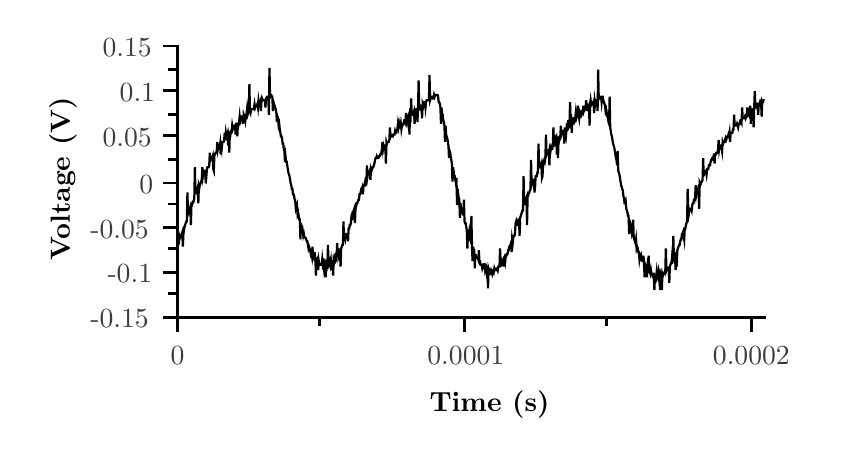
\begin{tikzpicture}{0pt}{0pt}{299pt}{150pt}
	\clip(0pt,150pt) -- (284.325pt,150pt) -- (284.325pt,7.36184pt) -- (0pt,7.36184pt) -- (0pt,150pt);
\begin{scope}
	\clip(54.2025pt,143.344pt) -- (266.258pt,143.344pt) -- (266.258pt,45.3987pt) -- (54.2025pt,45.3987pt) -- (54.2025pt,143.344pt);
	\color[gray]{0}
	\draw[line width=0.8pt, line join=miter, line cap=rect](54.4098pt,71.5173pt) -- (54.6171pt,72.1703pt) -- (54.8244pt,74.7821pt) -- (55.0317pt,74.1292pt) -- (55.2389pt,74.7821pt) -- (55.4462pt,74.7821pt) -- (55.6535pt,75.4351pt) -- (55.8608pt,76.0881pt) -- (56.0681pt,70.8644pt) -- (56.2754pt,75.4351pt) -- (56.4827pt,76.741pt) -- (56.69pt,78.047pt) -- (56.8972pt,78.6999pt) -- (57.1045pt,79.3529pt) -- (57.3118pt,80.0059pt) -- (57.5191pt,80.0059pt) -- (57.7264pt,90.4533pt) -- (57.9337pt,82.6177pt) -- (58.141pt,83.2707pt) -- (58.3483pt,84.5766pt) -- (58.5555pt,84.5766pt) -- (58.7628pt,85.2296pt) -- (58.9701pt,78.6999pt) -- (59.1774pt,85.8826pt) -- (59.3847pt,85.8826pt) -- (59.592pt,86.5355pt) -- (59.7993pt,87.1885pt) -- (60.0066pt,87.1885pt) -- (60.2138pt,88.4944pt) -- (60.4211pt,99.5948pt) -- (60.6284pt,89.8004pt) -- (60.8357pt,91.7593pt) -- (61.043pt,91.7593pt) -- (61.2503pt,91.7593pt) -- (61.4576pt,92.4122pt) -- (61.6649pt,86.5355pt) -- (61.8721pt,93.0652pt) -- (62.0794pt,92.4122pt) -- (62.2867pt,93.7182pt) -- (62.494pt,93.7182pt) -- (62.7013pt,94.3711pt) -- (62.9086pt,95.0241pt) -- (63.1159pt,99.5948pt) -- (63.3232pt,96.33pt) -- (63.5304pt,97.6359pt) -- (63.7377pt,97.6359pt) -- (63.945pt,98.2889pt) -- (64.1523pt,98.2889pt) -- (64.3596pt,93.7182pt) -- (64.5669pt,96.33pt) -- (64.7742pt,98.9419pt) -- (64.9815pt,99.5948pt) -- (65.1888pt,99.5948pt) -- (65.396pt,99.5948pt) -- (65.6033pt,100.248pt) -- (65.8106pt,104.819pt) -- (66.0179pt,102.207pt) -- (66.2252pt,102.86pt) -- (66.4325pt,102.86pt) -- (66.6398pt,102.86pt) -- (66.8471pt,103.513pt) -- (67.0543pt,98.9419pt) -- (67.2616pt,98.2889pt) -- (67.4689pt,104.166pt) -- (67.6762pt,104.166pt) -- (67.8835pt,104.819pt) -- (68.0908pt,104.819pt) -- (68.2981pt,104.819pt) -- (68.5054pt,108.736pt) -- (68.7126pt,106.125pt) -- (68.9199pt,107.43pt) -- (69.1272pt,107.43pt) -- (69.3345pt,106.777pt) -- (69.5418pt,108.083pt) -- (69.7491pt,104.166pt) -- (69.9564pt,108.736pt) -- (70.1637pt,106.777pt) -- (70.3709pt,108.736pt) -- (70.5782pt,108.736pt) -- (70.7855pt,108.736pt) -- (70.9928pt,109.389pt) -- (71.2001pt,112.001pt) -- (71.4074pt,109.389pt) -- (71.6147pt,112.001pt) -- (71.822pt,110.695pt) -- (72.0292pt,111.348pt) -- (72.2365pt,112.001pt) -- (72.4438pt,107.43pt) -- (72.6511pt,112.654pt) -- (72.8584pt,104.819pt) -- (73.0657pt,112.654pt) -- (73.273pt,111.348pt) -- (73.4803pt,112.654pt) -- (73.6876pt,112.654pt) -- (73.8948pt,114.613pt) -- (74.1021pt,113.307pt) -- (74.3094pt,113.96pt) -- (74.5167pt,113.96pt) -- (74.724pt,114.613pt) -- (74.9313pt,114.613pt) -- (75.1386pt,111.348pt) -- (75.3459pt,115.266pt) -- (75.5531pt,115.266pt) -- (75.7604pt,110.695pt) -- (75.9677pt,115.266pt) -- (76.175pt,115.266pt) -- (76.3823pt,115.919pt) -- (76.5896pt,117.878pt) -- (76.7969pt,115.919pt) -- (77.0042pt,116.572pt) -- (77.2114pt,116.572pt) -- (77.4187pt,117.878pt) -- (77.626pt,117.878pt) -- (77.8333pt,115.266pt) -- (78.0406pt,118.531pt) -- (78.2479pt,117.878pt) -- (78.4552pt,117.878pt) -- (78.6625pt,116.572pt) -- (78.8697pt,118.531pt) -- (79.077pt,118.531pt) -- (79.2843pt,120.49pt) -- (79.4916pt,118.531pt) -- (79.6989pt,119.184pt) -- (79.9062pt,119.837pt) -- (80.1135pt,129.631pt) -- (80.3208pt,119.837pt) -- (80.528pt,119.184pt) -- (80.7353pt,120.49pt) -- (80.9426pt,120.49pt) -- (81.1499pt,120.49pt) -- (81.3572pt,120.49pt) -- (81.5645pt,120.49pt) -- (81.7718pt,121.143pt) -- (81.9791pt,122.449pt) -- (82.1863pt,121.143pt) -- (82.3936pt,121.796pt) -- (82.6009pt,121.796pt) -- (82.8082pt,121.796pt) -- (83.0155pt,122.449pt) -- (83.2228pt,121.143pt) -- (83.4301pt,123.755pt) -- (83.6374pt,122.449pt) -- (83.8447pt,122.449pt) -- (84.0519pt,123.102pt) -- (84.2592pt,119.837pt) -- (84.4665pt,123.102pt) -- (84.6738pt,124.408pt) -- (84.8811pt,123.755pt) -- (85.0884pt,123.755pt) -- (85.2957pt,123.755pt) -- (85.503pt,123.755pt) -- (85.7102pt,123.755pt) -- (85.9175pt,121.143pt) -- (86.1248pt,124.408pt) -- (86.3321pt,124.408pt) -- (86.5394pt,125.061pt) -- (86.7467pt,125.061pt) -- (86.954pt,125.061pt) -- (87.1613pt,118.531pt) -- (87.3685pt,135.508pt) -- (87.5758pt,125.061pt) -- (87.7831pt,125.713pt) -- (87.9904pt,125.713pt) -- (88.1977pt,125.061pt) -- (88.405pt,125.061pt) -- (88.6123pt,119.837pt) -- (88.8196pt,123.102pt) -- (89.0268pt,122.449pt) -- (89.2341pt,121.796pt) -- (89.4414pt,121.143pt) -- (89.6487pt,120.49pt) -- (89.856pt,119.184pt) -- (90.0633pt,115.919pt) -- (90.2706pt,117.878pt) -- (90.4779pt,117.225pt) -- (90.6851pt,114.613pt) -- (90.8924pt,115.266pt) -- (91.0997pt,113.307pt) -- (91.307pt,112.001pt) -- (91.5143pt,110.695pt) -- (91.7216pt,110.695pt) -- (91.9289pt,110.042pt) -- (92.1362pt,108.083pt) -- (92.3435pt,108.083pt) -- (92.5507pt,106.125pt) -- (92.758pt,105.472pt) -- (92.9653pt,101.554pt) -- (93.1726pt,103.513pt) -- (93.3799pt,101.554pt) -- (93.5872pt,101.554pt) -- (93.7945pt,100.248pt) -- (94.0018pt,98.9419pt) -- (94.209pt,97.6359pt) -- (94.4163pt,96.983pt) -- (94.6236pt,96.33pt) -- (94.8309pt,95.0241pt) -- (95.0382pt,93.7182pt) -- (95.2455pt,93.0652pt) -- (95.4528pt,91.7593pt) -- (95.6601pt,91.7593pt) -- (95.8673pt,89.8004pt) -- (96.0746pt,89.8004pt) -- (96.2819pt,89.1474pt) -- (96.4892pt,87.8415pt) -- (96.6965pt,87.1885pt) -- (96.9038pt,84.5766pt) -- (97.1111pt,85.2296pt) -- (97.3184pt,85.8826pt) -- (97.5256pt,82.6177pt) -- (97.7329pt,83.2707pt) -- (97.9402pt,81.9648pt) -- (98.1475pt,80.6588pt) -- (98.3548pt,80.6588pt) -- (98.5621pt,73.4762pt) -- (98.7694pt,79.3529pt) -- (98.9767pt,78.047pt) -- (99.1839pt,78.047pt) -- (99.3912pt,76.741pt) -- (99.5985pt,74.7821pt) -- (99.8058pt,75.4351pt) -- (100.013pt,74.1292pt) -- (100.22pt,74.1292pt) -- (100.428pt,74.1292pt) -- (100.635pt,73.4762pt) -- (100.842pt,72.8232pt) -- (101.05pt,72.8232pt) -- (101.257pt,71.5173pt) -- (101.464pt,70.2114pt) -- (101.671pt,70.8644pt) -- (101.879pt,70.2114pt) -- (102.086pt,69.5584pt) -- (102.293pt,68.2525pt) -- (102.501pt,68.9055pt) -- (102.708pt,67.5995pt) -- (102.915pt,70.8644pt) -- (103.122pt,66.9466pt) -- (103.33pt,67.5995pt) -- (103.537pt,66.9466pt) -- (103.744pt,68.9055pt) -- (103.952pt,66.2936pt) -- (104.159pt,60.4169pt) -- (104.366pt,66.9466pt) -- (104.573pt,65.6406pt) -- (104.781pt,66.2936pt) -- (104.988pt,62.3758pt) -- (105.195pt,65.6406pt) -- (105.403pt,64.3347pt) -- (105.61pt,64.3347pt) -- (105.817pt,64.3347pt) -- (106.024pt,64.3347pt) -- (106.232pt,64.3347pt) -- (106.439pt,66.2936pt) -- (106.646pt,64.3347pt) -- (106.854pt,64.9877pt) -- (107.061pt,63.0288pt) -- (107.268pt,64.9877pt) -- (107.475pt,64.3347pt) -- (107.683pt,59.7639pt) -- (107.89pt,64.3347pt) -- (108.097pt,63.6817pt) -- (108.305pt,64.3347pt) -- (108.512pt,71.5173pt) -- (108.719pt,64.3347pt) -- (108.926pt,64.9877pt) -- (109.134pt,65.6406pt) -- (109.341pt,64.3347pt) -- (109.548pt,65.6406pt) -- (109.756pt,62.3758pt) -- (109.963pt,65.6406pt) -- (110.17pt,65.6406pt) -- (110.377pt,60.4169pt) -- (110.585pt,66.2936pt) -- (110.792pt,65.6406pt) -- (110.999pt,66.9466pt) -- (111.207pt,66.2936pt) -- (111.414pt,67.5995pt) -- (111.621pt,66.9466pt) -- (111.829pt,72.1703pt) -- (112.036pt,68.2525pt) -- (112.243pt,68.9055pt) -- (112.45pt,68.9055pt) -- (112.658pt,65.6406pt) -- (112.865pt,70.2114pt) -- (113.072pt,63.6817pt) -- (113.28pt,70.2114pt) -- (113.487pt,70.8644pt) -- (113.694pt,71.5173pt) -- (113.901pt,71.5173pt) -- (114.109pt,80.0059pt) -- (114.316pt,72.8232pt) -- (114.523pt,74.1292pt) -- (114.731pt,73.4762pt) -- (114.938pt,75.4351pt) -- (115.145pt,75.4351pt) -- (115.352pt,75.4351pt) -- (115.56pt,75.4351pt) -- (115.767pt,72.8232pt) -- (115.974pt,77.394pt) -- (116.182pt,77.394pt) -- (116.389pt,78.6999pt) -- (116.596pt,78.6999pt) -- (116.803pt,79.3529pt) -- (117.011pt,81.9648pt) -- (117.218pt,82.6177pt) -- (117.425pt,81.9648pt) -- (117.633pt,83.2707pt) -- (117.84pt,83.9237pt) -- (118.047pt,84.5766pt) -- (118.254pt,79.3529pt) -- (118.462pt,84.5766pt) -- (118.669pt,85.2296pt) -- (118.876pt,86.5355pt) -- (119.084pt,86.5355pt) -- (119.291pt,87.1885pt) -- (119.498pt,87.8415pt) -- (119.705pt,87.8415pt) -- (119.913pt,89.8004pt) -- (120.12pt,89.8004pt) -- (120.327pt,90.4533pt) -- (120.535pt,91.7593pt) -- (120.742pt,91.7593pt) -- (120.949pt,92.4122pt) -- (121.156pt,89.8004pt) -- (121.364pt,93.0652pt) -- (121.571pt,93.0652pt) -- (121.778pt,93.0652pt) -- (121.986pt,94.3711pt) -- (122.193pt,93.7182pt) -- (122.4pt,94.3711pt) -- (122.607pt,100.248pt) -- (122.815pt,96.33pt) -- (123.022pt,97.6359pt) -- (123.229pt,97.6359pt) -- (123.437pt,97.6359pt) -- (123.644pt,98.2889pt) -- (123.851pt,95.0241pt) -- (124.058pt,98.9419pt) -- (124.266pt,98.2889pt) -- (124.473pt,98.9419pt) -- (124.68pt,99.5948pt) -- (124.888pt,99.5948pt) -- (125.095pt,100.248pt) -- (125.302pt,100.901pt) -- (125.509pt,102.207pt) -- (125.717pt,102.86pt) -- (125.924pt,102.86pt) -- (126.131pt,103.513pt) -- (126.339pt,102.86pt) -- (126.546pt,102.86pt) -- (126.753pt,102.86pt) -- (126.961pt,103.513pt) -- (127.168pt,103.513pt) -- (127.375pt,104.166pt) -- (127.582pt,104.166pt) -- (127.79pt,104.819pt) -- (127.997pt,106.125pt) -- (128.204pt,108.736pt) -- (128.412pt,106.125pt) -- (128.619pt,107.43pt) -- (128.826pt,106.777pt) -- (129.033pt,107.43pt) -- (129.241pt,107.43pt) -- (129.448pt,100.901pt) -- (129.655pt,108.736pt) -- (129.863pt,108.083pt) -- (130.07pt,108.736pt) -- (130.277pt,108.736pt) -- (130.484pt,108.736pt) -- (130.692pt,109.389pt) -- (130.899pt,113.96pt) -- (131.106pt,110.695pt) -- (131.314pt,111.348pt) -- (131.521pt,111.348pt) -- (131.728pt,110.695pt) -- (131.935pt,110.695pt) -- (132.143pt,111.348pt) -- (132.35pt,111.348pt) -- (132.557pt,111.348pt) -- (132.765pt,112.654pt) -- (132.972pt,112.001pt) -- (133.179pt,112.001pt) -- (133.386pt,112.654pt) -- (133.594pt,113.307pt) -- (133.801pt,115.266pt) -- (134.008pt,113.96pt) -- (134.216pt,115.266pt) -- (134.423pt,113.96pt) -- (134.63pt,113.96pt) -- (134.837pt,115.266pt) -- (135.045pt,113.307pt) -- (135.252pt,114.613pt) -- (135.459pt,114.613pt) -- (135.667pt,115.266pt) -- (135.874pt,115.266pt) -- (136.081pt,116.572pt) -- (136.288pt,116.572pt) -- (136.496pt,115.919pt) -- (136.703pt,119.184pt) -- (136.91pt,117.225pt) -- (137.118pt,115.919pt) -- (137.325pt,117.225pt) -- (137.532pt,117.878pt) -- (137.739pt,118.531pt) -- (137.947pt,111.348pt) -- (138.154pt,118.531pt) -- (138.361pt,117.878pt) -- (138.569pt,124.408pt) -- (138.776pt,118.531pt) -- (138.983pt,118.531pt) -- (139.19pt,118.531pt) -- (139.398pt,119.184pt) -- (139.605pt,119.837pt) -- (139.812pt,115.266pt) -- (140.02pt,119.837pt) -- (140.227pt,119.837pt) -- (140.434pt,120.49pt) -- (140.642pt,120.49pt) -- (140.849pt,115.919pt) -- (141.056pt,121.143pt) -- (141.263pt,130.937pt) -- (141.471pt,121.143pt) -- (141.678pt,121.796pt) -- (141.885pt,121.143pt) -- (142.093pt,121.796pt) -- (142.3pt,121.796pt) -- (142.507pt,117.225pt) -- (142.714pt,122.449pt) -- (142.922pt,121.796pt) -- (143.129pt,123.102pt) -- (143.336pt,123.102pt) -- (143.544pt,123.102pt) -- (143.751pt,121.143pt) -- (143.958pt,123.102pt) -- (144.165pt,123.755pt) -- (144.373pt,123.755pt) -- (144.58pt,123.755pt) -- (144.787pt,123.755pt) -- (144.995pt,123.755pt) -- (145.202pt,132.896pt) -- (145.409pt,123.755pt) -- (145.616pt,124.408pt) -- (145.824pt,125.061pt) -- (146.031pt,125.061pt) -- (146.238pt,125.061pt) -- (146.446pt,124.408pt) -- (146.653pt,124.408pt) -- (146.86pt,125.713pt) -- (147.067pt,125.061pt) -- (147.275pt,125.713pt) -- (147.482pt,125.713pt) -- (147.689pt,125.713pt) -- (147.897pt,125.713pt) -- (148.104pt,125.713pt) -- (148.311pt,125.061pt) -- (148.518pt,123.102pt) -- (148.726pt,123.102pt) -- (148.933pt,122.449pt) -- (149.14pt,121.143pt) -- (149.348pt,115.266pt) -- (149.555pt,121.143pt) -- (149.762pt,118.531pt) -- (149.969pt,118.531pt) -- (150.177pt,116.572pt) -- (150.384pt,115.919pt) -- (150.591pt,114.613pt) -- (150.799pt,108.736pt) -- (151.006pt,114.613pt) -- (151.213pt,111.348pt) -- (151.42pt,110.695pt) -- (151.628pt,110.042pt) -- (151.835pt,108.736pt) -- (152.042pt,107.43pt) -- (152.25pt,102.86pt) -- (152.457pt,105.472pt) -- (152.664pt,104.819pt) -- (152.871pt,103.513pt) -- (153.079pt,102.207pt) -- (153.286pt,100.901pt) -- (153.493pt,94.3711pt) -- (153.701pt,99.5948pt) -- (153.908pt,98.2889pt) -- (154.115pt,96.33pt) -- (154.322pt,96.33pt) -- (154.53pt,95.0241pt) -- (154.737pt,93.7182pt) -- (154.944pt,95.6771pt) -- (155.152pt,85.8826pt) -- (155.359pt,91.7593pt) -- (155.566pt,89.8004pt) -- (155.774pt,88.4944pt) -- (155.981pt,87.8415pt) -- (156.188pt,81.3118pt) -- (156.395pt,86.5355pt) -- (156.603pt,84.5766pt) -- (156.81pt,84.5766pt) -- (157.017pt,83.2707pt) -- (157.225pt,82.6177pt) -- (157.432pt,82.6177pt) -- (157.639pt,87.8415pt) -- (157.846pt,80.0059pt) -- (158.054pt,79.3529pt) -- (158.261pt,79.3529pt) -- (158.468pt,78.047pt) -- (158.676pt,76.741pt) -- (158.883pt,70.2114pt) -- (159.09pt,75.4351pt) -- (159.297pt,74.7821pt) -- (159.505pt,76.0881pt) -- (159.712pt,73.4762pt) -- (159.919pt,73.4762pt) -- (160.127pt,72.8232pt) -- (160.334pt,81.9648pt) -- (160.541pt,71.5173pt) -- (160.748pt,65.6406pt) -- (160.956pt,70.8644pt) -- (161.163pt,69.5584pt) -- (161.37pt,69.5584pt) -- (161.578pt,63.0288pt) -- (161.785pt,68.2525pt) -- (161.992pt,66.9466pt) -- (162.199pt,66.9466pt) -- (162.407pt,66.9466pt) -- (162.614pt,66.9466pt) -- (162.821pt,66.2936pt) -- (163.029pt,69.5584pt) -- (163.236pt,65.6406pt) -- (163.443pt,65.6406pt) -- (163.65pt,64.3347pt) -- (163.858pt,64.3347pt) -- (164.065pt,64.3347pt) -- (164.272pt,63.0288pt) -- (164.48pt,63.6817pt) -- (164.687pt,63.0288pt) -- (164.894pt,63.0288pt) -- (165.101pt,64.9877pt) -- (165.309pt,62.3758pt) -- (165.516pt,63.0288pt) -- (165.723pt,61.7228pt) -- (165.931pt,63.0288pt) -- (166.138pt,62.3758pt) -- (166.345pt,55.8461pt) -- (166.552pt,63.0288pt) -- (166.76pt,62.3758pt) -- (166.967pt,62.3758pt) -- (167.174pt,61.7228pt) -- (167.382pt,62.3758pt) -- (167.589pt,61.7228pt) -- (167.796pt,61.0699pt) -- (168.003pt,62.3758pt) -- (168.211pt,62.3758pt) -- (168.418pt,61.7228pt) -- (168.625pt,63.0288pt) -- (168.833pt,62.3758pt) -- (169.04pt,62.3758pt) -- (169.247pt,62.3758pt) -- (169.455pt,63.0288pt) -- (169.662pt,63.0288pt) -- (169.869pt,62.3758pt) -- (170.076pt,63.6817pt) -- (170.284pt,63.6817pt) -- (170.491pt,63.6817pt) -- (170.698pt,70.2114pt) -- (170.906pt,63.6817pt) -- (171.113pt,64.9877pt) -- (171.32pt,65.6406pt) -- (171.527pt,64.9877pt) -- (171.735pt,65.6406pt) -- (171.942pt,63.6817pt) -- (172.149pt,66.2936pt) -- (172.357pt,66.9466pt) -- (172.564pt,65.6406pt) -- (172.771pt,67.5995pt) -- (172.978pt,67.5995pt) -- (173.186pt,68.2525pt) -- (173.393pt,68.2525pt) -- (173.6pt,69.5584pt) -- (173.808pt,69.5584pt) -- (174.015pt,70.8644pt) -- (174.222pt,70.8644pt) -- (174.429pt,71.5173pt) -- (174.637pt,72.1703pt) -- (174.844pt,68.9055pt) -- (175.051pt,73.4762pt) -- (175.259pt,72.1703pt) -- (175.466pt,74.1292pt) -- (175.673pt,74.7821pt) -- (175.88pt,74.7821pt) -- (176.088pt,75.4351pt) -- (176.295pt,79.3529pt) -- (176.502pt,80.0059pt) -- (176.71pt,78.6999pt) -- (176.917pt,78.6999pt) -- (177.124pt,79.3529pt) -- (177.331pt,80.6588pt) -- (177.539pt,80.6588pt) -- (177.746pt,74.7821pt) -- (177.953pt,81.3118pt) -- (178.161pt,81.9648pt) -- (178.368pt,82.6177pt) -- (178.575pt,83.2707pt) -- (178.782pt,83.9237pt) -- (178.99pt,83.9237pt) -- (179.197pt,96.33pt) -- (179.404pt,85.8826pt) -- (179.612pt,87.1885pt) -- (179.819pt,87.1885pt) -- (180.026pt,87.8415pt) -- (180.233pt,88.4944pt) -- (180.441pt,78.6999pt) -- (180.648pt,89.1474pt) -- (180.855pt,89.1474pt) -- (181.063pt,90.4533pt) -- (181.27pt,90.4533pt) -- (181.477pt,91.1063pt) -- (181.684pt,91.7593pt) -- (181.892pt,102.207pt) -- (182.099pt,93.0652pt) -- (182.306pt,93.7182pt) -- (182.514pt,94.3711pt) -- (182.721pt,95.0241pt) -- (182.928pt,95.0241pt) -- (183.135pt,90.4533pt) -- (183.343pt,92.4122pt) -- (183.55pt,96.33pt) -- (183.757pt,96.33pt) -- (183.965pt,96.33pt) -- (184.172pt,97.6359pt) -- (184.379pt,97.6359pt) -- (184.587pt,108.083pt) -- (184.794pt,99.5948pt) -- (185.001pt,99.5948pt) -- (185.208pt,100.248pt) -- (185.416pt,100.248pt) -- (185.623pt,100.901pt) -- (185.83pt,95.6771pt) -- (186.038pt,96.33pt) -- (186.245pt,100.901pt) -- (186.452pt,101.554pt) -- (186.659pt,102.207pt) -- (186.867pt,101.554pt) -- (187.074pt,102.86pt) -- (187.281pt,111.348pt) -- (187.489pt,104.166pt) -- (187.696pt,104.819pt) -- (187.903pt,104.819pt) -- (188.11pt,104.819pt) -- (188.318pt,105.472pt) -- (188.525pt,100.248pt) -- (188.732pt,106.125pt) -- (188.94pt,105.472pt) -- (189.147pt,106.777pt) -- (189.354pt,106.125pt) -- (189.561pt,106.125pt) -- (189.769pt,107.43pt) -- (189.976pt,113.96pt) -- (190.183pt,107.43pt) -- (190.391pt,111.348pt) -- (190.598pt,108.736pt) -- (190.805pt,109.389pt) -- (191.012pt,110.042pt) -- (191.22pt,104.166pt) -- (191.427pt,110.042pt) -- (191.634pt,102.86pt) -- (191.842pt,110.695pt) -- (192.049pt,109.389pt) -- (192.256pt,110.695pt) -- (192.463pt,110.695pt) -- (192.671pt,114.613pt) -- (192.878pt,111.348pt) -- (193.085pt,112.001pt) -- (193.293pt,112.001pt) -- (193.5pt,112.654pt) -- (193.707pt,112.654pt) -- (193.914pt,108.083pt) -- (194.122pt,113.96pt) -- (194.329pt,112.654pt) -- (194.536pt,111.348pt) -- (194.744pt,113.96pt) -- (194.951pt,113.307pt) -- (195.158pt,113.96pt) -- (195.365pt,116.572pt) -- (195.573pt,114.613pt) -- (195.78pt,115.266pt) -- (195.987pt,123.102pt) -- (196.195pt,115.919pt) -- (196.402pt,116.572pt) -- (196.609pt,112.001pt) -- (196.816pt,116.572pt) -- (197.024pt,115.919pt) -- (197.231pt,116.572pt) -- (197.438pt,115.919pt) -- (197.646pt,116.572pt) -- (197.853pt,117.225pt) -- (198.06pt,119.184pt) -- (198.268pt,117.225pt) -- (198.475pt,117.878pt) -- (198.682pt,117.878pt) -- (198.889pt,121.796pt) -- (199.097pt,118.531pt) -- (199.304pt,117.225pt) -- (199.511pt,119.184pt) -- (199.719pt,118.531pt) -- (199.926pt,119.184pt) -- (200.133pt,118.531pt) -- (200.34pt,119.184pt) -- (200.548pt,119.184pt) -- (200.755pt,121.796pt) -- (200.962pt,119.837pt) -- (201.17pt,120.49pt) -- (201.377pt,120.49pt) -- (201.584pt,120.49pt) -- (201.791pt,123.755pt) -- (201.999pt,119.837pt) -- (202.206pt,121.796pt) -- (202.413pt,121.143pt) -- (202.621pt,121.143pt) -- (202.828pt,121.796pt) -- (203.035pt,114.613pt) -- (203.242pt,121.796pt) -- (203.45pt,123.755pt) -- (203.657pt,122.449pt) -- (203.864pt,123.102pt) -- (204.072pt,123.102pt) -- (204.279pt,122.449pt) -- (204.486pt,123.102pt) -- (204.693pt,119.184pt) -- (204.901pt,123.755pt) -- (205.108pt,122.449pt) -- (205.315pt,123.755pt) -- (205.523pt,123.755pt) -- (205.73pt,123.755pt) -- (205.937pt,119.837pt) -- (206.144pt,134.855pt) -- (206.352pt,124.408pt) -- (206.559pt,125.061pt) -- (206.766pt,125.061pt) -- (206.974pt,125.061pt) -- (207.181pt,125.061pt) -- (207.388pt,123.102pt) -- (207.595pt,125.061pt) -- (207.803pt,125.061pt) -- (208.01pt,123.755pt) -- (208.217pt,123.102pt) -- (208.425pt,122.449pt) -- (208.632pt,121.796pt) -- (208.839pt,119.837pt) -- (209.046pt,120.49pt) -- (209.254pt,119.184pt) -- (209.461pt,117.878pt) -- (209.668pt,117.878pt) -- (209.876pt,115.919pt) -- (210.083pt,115.266pt) -- (210.29pt,125.061pt) -- (210.497pt,113.96pt) -- (210.705pt,112.654pt) -- (210.912pt,111.348pt) -- (211.119pt,110.695pt) -- (211.327pt,109.389pt) -- (211.534pt,108.083pt) -- (211.741pt,107.43pt) -- (211.948pt,106.777pt) -- (212.156pt,105.472pt) -- (212.363pt,104.166pt) -- (212.57pt,102.86pt) -- (212.778pt,102.207pt) -- (212.985pt,100.248pt) -- (213.192pt,105.472pt) -- (213.4pt,98.2889pt) -- (213.607pt,97.6359pt) -- (213.814pt,96.983pt) -- (214.021pt,95.6771pt) -- (214.229pt,94.3711pt) -- (214.436pt,93.0652pt) -- (214.643pt,92.4122pt) -- (214.851pt,91.7593pt) -- (215.058pt,91.1063pt) -- (215.265pt,89.1474pt) -- (215.472pt,88.4944pt) -- (215.68pt,86.5355pt) -- (215.887pt,86.5355pt) -- (216.094pt,87.1885pt) -- (216.302pt,84.5766pt) -- (216.509pt,83.9237pt) -- (216.716pt,83.2707pt) -- (216.923pt,81.9648pt) -- (217.131pt,81.9648pt) -- (217.338pt,75.4351pt) -- (217.545pt,80.0059pt) -- (217.753pt,79.3529pt) -- (217.96pt,78.047pt) -- (218.167pt,77.394pt) -- (218.374pt,75.4351pt) -- (218.582pt,76.0881pt) -- (218.789pt,80.6588pt) -- (218.996pt,74.1292pt) -- (219.204pt,73.4762pt) -- (219.411pt,72.8232pt) -- (219.618pt,72.1703pt) -- (219.825pt,73.4762pt) -- (220.033pt,70.2114pt) -- (220.24pt,70.8644pt) -- (220.447pt,70.2114pt) -- (220.655pt,68.9055pt) -- (220.862pt,68.9055pt) -- (221.069pt,66.2936pt) -- (221.276pt,67.5995pt) -- (221.484pt,66.9466pt) -- (221.691pt,67.5995pt) -- (221.898pt,66.2936pt) -- (222.106pt,65.6406pt) -- (222.313pt,65.6406pt) -- (222.52pt,67.5995pt) -- (222.727pt,64.3347pt) -- (222.935pt,59.7639pt) -- (223.142pt,64.3347pt) -- (223.349pt,63.6817pt) -- (223.557pt,63.0288pt) -- (223.764pt,59.7639pt) -- (223.971pt,63.0288pt) -- (224.178pt,61.7228pt) -- (224.386pt,67.5995pt) -- (224.593pt,61.7228pt) -- (224.8pt,61.7228pt) -- (225.008pt,61.0699pt) -- (225.215pt,62.3758pt) -- (225.422pt,61.0699pt) -- (225.629pt,61.0699pt) -- (225.837pt,60.4169pt) -- (226.044pt,61.0699pt) -- (226.251pt,61.0699pt) -- (226.459pt,55.1932pt) -- (226.666pt,60.4169pt) -- (226.873pt,60.4169pt) -- (227.081pt,59.7639pt) -- (227.288pt,61.7228pt) -- (227.495pt,59.7639pt) -- (227.702pt,60.4169pt) -- (227.91pt,61.7228pt) -- (228.117pt,59.7639pt) -- (228.324pt,61.0699pt) -- (228.532pt,55.1932pt) -- (228.739pt,61.0699pt) -- (228.946pt,60.4169pt) -- (229.153pt,55.1932pt) -- (229.361pt,61.0699pt) -- (229.568pt,60.4169pt) -- (229.775pt,61.0699pt) -- (229.983pt,61.0699pt) -- (230.19pt,61.7228pt) -- (230.397pt,61.7228pt) -- (230.604pt,70.2114pt) -- (230.812pt,62.3758pt) -- (231.019pt,63.0288pt) -- (231.226pt,62.3758pt) -- (231.434pt,62.3758pt) -- (231.641pt,63.6817pt) -- (231.848pt,57.805pt) -- (232.055pt,63.6817pt) -- (232.263pt,64.3347pt) -- (232.47pt,64.9877pt) -- (232.677pt,64.9877pt) -- (232.885pt,67.5995pt) -- (233.092pt,66.2936pt) -- (233.299pt,74.7821pt) -- (233.506pt,66.9466pt) -- (233.714pt,67.5995pt) -- (233.921pt,67.5995pt) -- (234.128pt,62.3758pt) -- (234.336pt,68.9055pt) -- (234.543pt,63.6817pt) -- (234.75pt,69.5584pt) -- (234.957pt,70.2114pt) -- (235.165pt,70.8644pt) -- (235.372pt,71.5173pt) -- (235.579pt,71.5173pt) -- (235.787pt,72.8232pt) -- (235.994pt,73.4762pt) -- (236.201pt,73.4762pt) -- (236.408pt,75.4351pt) -- (236.616pt,75.4351pt) -- (236.823pt,76.0881pt) -- (237.03pt,74.7821pt) -- (237.238pt,73.4762pt) -- (237.445pt,77.394pt) -- (237.652pt,77.394pt) -- (237.859pt,78.6999pt) -- (238.067pt,79.3529pt) -- (238.274pt,80.0059pt) -- (238.481pt,91.7593pt) -- (238.689pt,84.5766pt) -- (238.896pt,82.6177pt) -- (239.103pt,83.9237pt) -- (239.31pt,84.5766pt) -- (239.518pt,84.5766pt) -- (239.725pt,84.5766pt) -- (239.932pt,83.9237pt) -- (240.14pt,85.8826pt) -- (240.347pt,86.5355pt) -- (240.554pt,86.5355pt) -- (240.761pt,87.8415pt) -- (240.969pt,87.8415pt) -- (241.176pt,88.4944pt) -- (241.383pt,93.0652pt) -- (241.591pt,89.8004pt) -- (241.798pt,91.1063pt) -- (242.005pt,91.7593pt) -- (242.213pt,91.7593pt) -- (242.42pt,92.4122pt) -- (242.627pt,84.5766pt) -- (242.834pt,93.7182pt) -- (243.042pt,93.0652pt) -- (243.249pt,93.7182pt) -- (243.456pt,94.3711pt) -- (243.664pt,94.3711pt) -- (243.871pt,95.0241pt) -- (244.078pt,102.86pt) -- (244.285pt,96.33pt) -- (244.493pt,97.6359pt) -- (244.7pt,97.6359pt) -- (244.907pt,98.2889pt) -- (245.115pt,98.2889pt) -- (245.322pt,96.983pt) -- (245.529pt,98.9419pt) -- (245.736pt,98.9419pt) -- (245.944pt,98.9419pt) -- (246.151pt,100.248pt) -- (246.358pt,100.248pt) -- (246.566pt,100.248pt) -- (246.773pt,101.554pt) -- (246.98pt,102.207pt) -- (247.187pt,102.207pt) -- (247.395pt,102.86pt) -- (247.602pt,102.86pt) -- (247.809pt,103.513pt) -- (248.017pt,102.86pt) -- (248.224pt,100.901pt) -- (248.431pt,104.166pt) -- (248.638pt,104.166pt) -- (248.846pt,104.819pt) -- (249.053pt,104.819pt) -- (249.26pt,104.819pt) -- (249.468pt,106.125pt) -- (249.675pt,109.389pt) -- (249.882pt,106.125pt) -- (250.089pt,107.43pt) -- (250.297pt,107.43pt) -- (250.504pt,107.43pt) -- (250.711pt,106.777pt) -- (250.919pt,105.472pt) -- (251.126pt,108.736pt) -- (251.333pt,108.083pt) -- (251.54pt,108.736pt) -- (251.748pt,108.736pt) -- (251.955pt,109.389pt) -- (252.162pt,110.042pt) -- (252.37pt,109.389pt) -- (252.577pt,110.042pt) -- (252.784pt,110.695pt) -- (252.991pt,110.695pt) -- (253.199pt,111.348pt) -- (253.406pt,110.695pt) -- (253.613pt,112.001pt) -- (253.821pt,108.736pt) -- (254.028pt,112.001pt) -- (254.235pt,112.001pt) -- (254.442pt,112.001pt) -- (254.65pt,112.001pt) -- (254.857pt,113.307pt) -- (255.064pt,113.307pt) -- (255.272pt,118.531pt) -- (255.479pt,114.613pt) -- (255.686pt,114.613pt) -- (255.894pt,114.613pt) -- (256.101pt,114.613pt) -- (256.308pt,115.266pt) -- (256.515pt,114.613pt) -- (256.723pt,113.96pt) -- (256.93pt,115.266pt) -- (257.137pt,115.266pt) -- (257.345pt,115.266pt) -- (257.552pt,116.572pt) -- (257.759pt,116.572pt) -- (257.966pt,115.919pt) -- (258.174pt,121.143pt) -- (258.381pt,117.225pt) -- (258.588pt,117.225pt) -- (258.796pt,117.225pt) -- (259.003pt,117.225pt) -- (259.21pt,117.878pt) -- (259.417pt,117.225pt) -- (259.625pt,117.878pt) -- (259.832pt,117.878pt) -- (260.039pt,121.143pt) -- (260.247pt,119.184pt) -- (260.454pt,119.184pt) -- (260.661pt,118.531pt) -- (260.868pt,119.184pt) -- (261.076pt,121.796pt) -- (261.283pt,115.266pt) -- (261.49pt,119.837pt) -- (261.698pt,120.49pt) -- (261.905pt,120.49pt) -- (262.112pt,120.49pt) -- (262.319pt,113.96pt) -- (262.527pt,121.143pt) -- (262.734pt,127.019pt) -- (262.941pt,121.796pt) -- (263.149pt,121.143pt) -- (263.356pt,121.143pt) -- (263.563pt,121.796pt) -- (263.77pt,121.143pt) -- (263.978pt,118.531pt) -- (264.185pt,122.449pt) -- (264.392pt,122.449pt) -- (264.6pt,123.102pt) -- (264.807pt,122.449pt) -- (265.014pt,123.102pt) -- (265.221pt,117.878pt) -- (265.429pt,123.102pt) -- (265.636pt,123.102pt) -- (265.843pt,123.755pt) -- (266.051pt,123.755pt) -- (266.258pt,123.755pt);
\end{scope}
\begin{scope}
	\color[gray]{0}
	\pgftext[center, base, at={\pgfpoint{15.2147pt}{95.3146pt}},rotate=90]{\textbf{Voltage (V)}}
	\color[gray]{0.235294}
	\pgftext[center, base, at={\pgfpoint{33.2154pt}{41.595pt}}]{-0.15}
	\pgftext[center, base, at={\pgfpoint{36.9076pt}{57.7607pt}}]{-0.1}
	\pgftext[center, base, at={\pgfpoint{33.2154pt}{73.9263pt}}]{-0.05}
	\pgftext[center, base, at={\pgfpoint{42.9029pt}{90.092pt}}]{0}
	\pgftext[center, base, at={\pgfpoint{35.9567pt}{107.209pt}}]{0.05}
	\pgftext[center, base, at={\pgfpoint{39.649pt}{123.374pt}}]{0.1}
	\pgftext[center, base, at={\pgfpoint{35.9567pt}{139.54pt}}]{0.15}
	\color[gray]{0}
	\draw[line width=1pt, line join=bevel, line cap=rect](54.2025pt,53.957pt) -- (51.3497pt,53.957pt);
	\draw[line width=1pt, line join=bevel, line cap=rect](54.2025pt,70.1226pt) -- (51.3497pt,70.1226pt);
	\draw[line width=1pt, line join=bevel, line cap=rect](54.2025pt,86.2883pt) -- (51.3497pt,86.2883pt);
	\draw[line width=1pt, line join=bevel, line cap=rect](54.2025pt,102.454pt) -- (51.3497pt,102.454pt);
	\draw[line width=1pt, line join=bevel, line cap=rect](54.2025pt,118.62pt) -- (51.3497pt,118.62pt);
	\draw[line width=1pt, line join=bevel, line cap=rect](54.2025pt,134.785pt) -- (51.3497pt,134.785pt);
	\draw[line width=1pt, line join=bevel, line cap=rect](54.2025pt,45.3987pt) -- (49.4479pt,45.3987pt);
	\draw[line width=1pt, line join=bevel, line cap=rect](54.2025pt,61.5643pt) -- (49.4479pt,61.5643pt);
	\draw[line width=1pt, line join=bevel, line cap=rect](54.2025pt,77.73pt) -- (49.4479pt,77.73pt);
	\draw[line width=1pt, line join=bevel, line cap=rect](54.2025pt,93.8957pt) -- (49.4479pt,93.8957pt);
	\draw[line width=1pt, line join=bevel, line cap=rect](54.2025pt,111.012pt) -- (49.4479pt,111.012pt);
	\draw[line width=1pt, line join=bevel, line cap=rect](54.2025pt,127.178pt) -- (49.4479pt,127.178pt);
	\draw[line width=1pt, line join=bevel, line cap=rect](54.2025pt,143.344pt) -- (49.4479pt,143.344pt);
	\draw[line width=1pt, line join=bevel, line cap=rect](54.2025pt,143.344pt) -- (54.2025pt,45.3987pt);
	\pgftext[center, base, at={\pgfpoint{166.887pt}{11.1655pt}}]{\textbf{Time (s)}}
	\color[gray]{0.235294}
	\pgftext[center, base, at={\pgfpoint{54.1951pt}{28.2821pt}}]{0}
	\pgftext[center, base, at={\pgfpoint{158.328pt}{28.2821pt}}]{0.0001}
	\pgftext[center, base, at={\pgfpoint{261.503pt}{28.2821pt}}]{0.0002}
	\color[gray]{0}
	\draw[line width=1pt, line join=bevel, line cap=rect](105.552pt,45.3987pt) -- (105.552pt,42.5459pt);
	\draw[line width=1pt, line join=bevel, line cap=rect](209.203pt,45.3987pt) -- (209.203pt,42.5459pt);
	\draw[line width=1pt, line join=bevel, line cap=rect](54.2025pt,45.3987pt) -- (54.2025pt,40.6441pt);
	\draw[line width=1pt, line join=bevel, line cap=rect](157.853pt,45.3987pt) -- (157.853pt,40.6441pt);
	\draw[line width=1pt, line join=bevel, line cap=rect](261.503pt,45.3987pt) -- (261.503pt,40.6441pt);
	\draw[line width=1pt, line join=bevel, line cap=rect](54.2025pt,45.3987pt) -- (266.258pt,45.3987pt);
\end{scope}
\end{tikzpicture}

		\caption{New signal produced when the two 7555 chips are used in the circuit and combined by the mixer.}
		\label{fig:7555}
\end{figure}

\subsection{Mixer - SA612A}
\label{sec:SA612A-mixer}
The mixer chip is used to calculate the difference in frequency between the input signals and output this difference as a new signal. This allows a small influence to the circuit to cause a big difference in the signal by comparing two high frequency inputs so that the relative difference is large. The chip that is used is the SA612A IC which is a double-balanced mixer and oscillator\cite{SA612A}. The pin configuration and internal block configuration is shown in appendix~\ref{app:SA612A}. This particular mixer chip subtracts the lower frequency signal from the higher one to give a simple difference relation.

The chip is tested using a pair of TG315 signal generators to provide a known input frequency that can be used to examine the performance of the mixer chip. It is found, when using this set-up, that though the output signal is the difference between the inputs, as expected, the signal is not perfectly clean, and there is a considerable amount of high frequency noise left. This produces a unpleasant rough high pitched addition to the sound. This is required to be removed in order that the instrument be acceptable to listen to. These unwanted parts of the signal shall be removed using a low pass filter.

\subsection{Low Pass Filter}
\label{sec:lowpass}
A low pass filter is a circuit whose output depends on the frequency of the input. The circuit has a cut off frequency, above which the amplitude of the signal is severely attenuated. This cut-off can be chosen depending on the components used. This allows the high frequency noise to be removed whilst leaving the important signal largely unaffected.

The low pass filter is composed of a resistor and a capacitor to ground, as shown in figure~\ref{fig:low_pass}. The capacitor acts as an open circuit at low frequency signals, so these parts are not affected, but acts as a short circuit at high frequencies, so these pass to ground and hence are removed from signal. To satisfactorily remove the noise, two low pass filters are placed in series with a $\times 1$ buffer amplifier between them. This produces a sharper cut-off so that less of the important signal is lost. The buffer amplifier is added to ensure the two filters are isolated from each other. It is formed of an operational-amplifier (op-amp) with the output fed back into the inverting input. The op-amp used is the LT081 operational amplifier, described in appendix~\ref{app:lt081}.

\begin{figure}[htbp]
	\begin{center}
		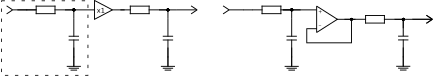
\includegraphics[width=\textwidth]{report_img/buffer_amp}
		\caption{The low pass filter is an extremely simple circuit to remove unwanted high frequency noise. The circuit on the left shows the principle of having two low pass filters separated by a $\times 1$ buffer amplifier, with the single low pass filter highlighted. The second circuit shows the implementation of the op-amp bases buffer.}
		\label{fig:low_pass}
	\end{center}
\end{figure}

The approximate frequency of the cut-off of the low pass filter is given by the equation
\begin{equation}
	f_c = \frac{1}{2\pi RC},
\end{equation}
where $R$ is the resistor and $C$ is the capacitor in the previous circuit. A cut-off of around 20\,kHz is desired, corresponding to the upper limit of human hearing, and so a resistor of 820\,$\Omega$ and capacitor of 10\,nF is used. Equation~\ref{eqn:low pass numbers} shows that this gives a value that is very close to the desired value,
\begin{equation}
		f_c \frac{1}{2\pi\times 820 \times 10 \times 10^{-9}} = 19,409\,\text{Hz}.
		\label{eqn:low pass numbers}
\end{equation}
The resulting signal is much cleaner in the high frequency range and so much more pleasant to listen to. A comparison of the signal before and after the low pass filter is shown in figure~\ref{fig:filter before after}.

\begin{figure}[htbp]
	\centering
		\input{report_img/before_after_filter.tex} 
		\vspace{-10pt}
		\caption{The signal before the low pass filter, left, and after, right. Only the high frequency oscillations are affected leaving the envelope signal unchanged, but cleaner.}
		\label{fig:filter before after}
\end{figure}

\subsection{Parallel Plate Capacitor}
\label{sec:PPCapacitor}
The main attraction of the theremin is the novel control of the instrument remotely. This is achieved using a parallel plate capacitor. A capacitor is "a device used to store an electrical charge, consisting of one or more pairs of conductors separated by an insulator"\cite{OED2000}. When used in the theremin, one of the conductors is the user, via their hand which is closest to the instrument, and the other is the aerial connected to the circuit; the insulator is the air in between them. 

The aerial used to test the theremin, is a square of metal of known dimensions, insulated from, and suspended by a retort stand. The definite size of this piece of equipment allows the capacitance to be estimated from the simple capacitor equation (equation~(\ref{eqn:capacitor})). The plate capacitor is connected to the VCO that controls the pitch. For a complete theremin, there would be two separate plate capacitors, one for pitch and one for volume, but only one shall be used here for simplicity.

This set-up is used to produce the variation in frequency shown in figure~\ref{fig:capacitor high low}. Though this represents a definite change in the output frequency of the VCO, the change is too small to be heard. The shape of the wave is also not as expected since the high time and low time are not equal. This was expected to a small degree since the duty cycle of the chip is always less than 50\%, but not to the extent seen here.

\begin{figure}[htbp]
	\centering
		\input{report_img/capacitor_high_low.tex} 
		\caption{The change in frequency accessible by the plate capacitor. The original frequency, black, is when there is minimal external presence near the capacitor, and so a minuscule capacitance, compared with the maximum frequency possible, red, when a user's hand is placed directly next to, but not touching, the plate.}
		\label{fig:capacitor high low}
\end{figure}

The metal used for the aerial is roughly a square with sides $15\times 15\,\text{cm}$. The area of the average human hand is roughly $420\,\text{cm}^2$ and so the area concerned with the plate capacitor is about half of this value, $210\,\text{cm}^2$\cite{Joo-Young-Lee2007}. From this, it is possible to estimate a value for the capacitance provided by the parallel plate capacitor at different distances, as shown in equation~(\ref{eqn:cap0.03}) and (\ref{eqn:cap0.01})
\begin{align}
	\text{For } d = 0.3, \qquad C &= \frac{1\times 8.854\times 10^{-12} \times 0.021}{0.03} \label{eqn:cap0.03}\\
			&= 6.20\times 10^{-13}\,F \nonumber \\
	\text{For } d = 0.1, \qquad C &= \frac{1\times 8.854\times 10^{-12} \times 0.021}{0.01} \label{eqn:cap0.01}\\
			&= 1.86\times 10^{-12}\,F \nonumber
\end{align}
These values are extremely small capacitances to be measured by the standard components that are to be used whilst continuing to allow the finished instrument to be commercially viable. For the initial design with the 555 or 4046 chips, this change would be far too small to be detected. Only with the increase in frequency provided by the 7555 chip is this detection possible.

An attempt to increase the capacitance change caused by moving close to the plate is made by adding several separate fixed value capacitors in series with the variable capacitor. When in series, the total capacitance is given by the sum of the reciprocals of the separate capacitances. A sequence of four small 1\,nF capacitors is added in series with a total capacitance shown in equation~(\ref{eqn:capacitors in series}).
\begin{align}
	\frac{1}{C_\text{total}} &= \frac{1}{C_1}+\frac{1}{C_2}+\frac{1}{C_3}+\ldots+\frac{1}{C_N} \label{eqn:capacitors in series}\\
	C_\text{total} &= \left( 4\times \frac{1}{1\times 10^{-9}}\right)^{-1} \nonumber \\
	&= 250\,pF \nonumber
\end{align}

\newpage 
